% =====================================================================
% Chapter I.2: Observables I: local operators
% =====================================================================
\section{Observables I: local operators}
\label{ch:local-operators}

Chapter I.1 dismantled a definition and left an inventory in its place
(Definition~\ref{def:inventory}). This chapter makes the book's first
affirmative claim: the oldest entry of that inventory --- the local operators
and their correlation functions --- is \emph{primary data}. Local operators
are not records kept about a theory that truly lives in some Lagrangian; they
are the theory's observables in the fullest sense of
Idea~\ref{idea:observables}: data from which the rest of the theory's life on
$\reals^d$ --- states, dynamics, symmetries, the response to geometry --- can
be rebuilt, and whose precise limits, charted at the chapter's end, are what
the rest of Part I exists to cross. A claim like that has content only if
three debts are paid. One must say what a correlation function actually
\emph{is} --- in particular how the Euclidean correlators that lattices and
path integrals produce are related to the Lorentzian amplitudes that quantum
mechanics demands. One must show that correlators \emph{contain} the theory
--- that the Hilbert space, the Hamiltonian, and the operators themselves are
hiding inside $\langle \op_1 \cdots \op_n\rangle$, so that whoever specifies
consistent correlators has specified everything. And one must find structure
in the list: the set of all $n$-point functions of all operators is an
absurdly overdetermined, infinitely redundant presentation of anything, and
primary data is usable data only if the redundancy is organized by something
sharp. This chapter pays the three debts for pointlike operators --- and
discovers along the way that the three answers are one answer.

\begin{qquestion}
Are the local operators of a quantum field theory genuinely its
\emph{observables} --- primary data that determines the theory --- rather
than bookkeeping attached to a presentation? Concretely: in what sense do
correlators \emph{contain} states, operators, and a Hamiltonian; what
organizes the infinite list of correlation functions into usable data; and
which operators must every local theory contain?
\end{qquestion}

\noin The chapter's centerpiece is the operator product expansion. In the
quantum field theory you already know, the OPE is an asymptotic statement about
short distances, one further entry in the perturbative toolbox. In a conformal
field theory it is something else entirely: a \emph{convergent} expansion, valid
at finite separation, with a radius of convergence you can draw with a compass
--- and therefore an exact multiplication law on the space of local operators.
The modern subject leans on this fact constantly; the bootstrap of Part III is
nothing but this fact taken seriously. We will prove it, by a quantum-mechanical
argument (radial quantization) whose punchline deserves advance billing: the
reconstruction theorems, which build a Hilbert space out of Euclidean
correlators by cutting spacetime along planes, can be run just as well cutting
along \emph{spheres} --- and the OPE is then revealed as an ordinary expansion
of a state in a complete basis, convergent for the same reason Fourier series
are. The chapter closes with the two operators that locality forces on every
QFT --- the stress tensor and the conserved currents --- and with a worked
counterexample, the generalized free field, showing exactly what goes missing
when they are absent.

Throughout, ``the theory'' is presented however convenient --- lattice, path
integral, canonical --- in the spirit of chapter I.1: presentations are
scaffolding, and everything we establish is a statement about the correlators
themselves. But there is a question prior even to the three debts, one that
textbooks answer so implicitly that most readers never notice it being
answered: what, exactly, \emph{is} a local operator? Since this chapter
proposes to build theories out of these objects, we owe them a section first.

% =====================================================================
\subsection{First: what is a local operator?}
\label{sec:what-is-operator}

The inventory of chapter I.1 spoke of ``labels $\op_i$ drawn from a set of
local operators,'' and the phrase passed without comment. In a Lagrangian
presentation the implicit answer seems obvious: the local operators are the
field $\phi$, its derivatives, and local polynomials in them --- $\phi^2$,
$\phi^4$, $\phi\,\partial^2\phi$, and so on. The obvious answer is wrong twice
over, in instructive ways, and repairing it produces the concept this chapter
actually runs on.

\emph{It is wrong, first, because products at a point do not exist.} Take the
free massless scalar in $d = 4$ and try to define $\phi(x)^2$. Its expectation
value is $\langle \phi(x)\phi(x)\rangle = \lim_{\varepsilon\to0}
\frac{1}{4\pi^2 \varepsilon^2} = \infty$: the would-be operator has infinite
overlap with the identity. The repair is as old as the subject ---
\vocab{normal ordering}, better viewed as \emph{point-splitting}:
\begin{equation}
:\!\phi^2\!:(x) \;\equiv\; \lim_{\varepsilon \to 0}\,
\Big[\, \phi(x + \varepsilon)\,\phi(x) \;-\;
\big\langle \phi(x+\varepsilon)\,\phi(x)\big\rangle \,\Big],
\label{eq:point-splitting}
\end{equation}
subtract the singular part of the product, then collide the points. Notice
the shape of the repair: the singularity of a product of local operators was
itself proportional to a local operator (here, the identity), and a finite
operator emerged once that piece was removed. In an interacting theory the
same procedure needs more terms --- the product $\phi(x+\varepsilon)\phi(x)$
contains, alongside the identity, singular multiples of \emph{other} local
operators, all of which must be subtracted, and the surviving finite operators
\emph{mix} under changes of the splitting scale, which is how anomalous
dimensions enter. The reader should recognize what this is: the operator
product expansion, encountered backwards, as a renormalization procedure ---
Section~\ref{sec:ope} will run the same structure forwards, as an exact
expansion. The
``set of local operators'' of an interacting theory is not the classical
polynomial algebra; it is what survives this organizing of coincident-point
singularities --- smaller in some ways (in the free theory $\partial^2\phi =
0$: equations of motion are operator identities, and null operators must be
quotiented away), larger in others, and with its dimensions shifted away from
naive counting.

\emph{It is wrong, second, because the lattice knows nothing of $\phi$.} Take
instead the critical 2d Ising model, the lattice presentation of a CFT. What
is the local operator content there? The natural candidates are local
functions of nearby spins: $s_i$, or $s_i s_{i+1}$, or any finite cluster.
But these are not the operators with clean transformation properties ---
none of them scales homogeneously under coarse-graining. Wilson's
renormalization group supplies the right notion: linearize the RG around the
fixed point, and define the \vocab{scaling operators} $\op_\Delta$ as its
eigenvectors --- the special combinations that reproduce themselves, times
$\lambda^{-\Delta}$, under a zoom by $\lambda$. Expressed in lattice
variables, a scaling operator is an infinite sum with contributions of every
size,
\begin{equation}
\sigma(x_i) \;\sim\; s_i \,+\, (\text{three-spin terms}) \,+\,
(\text{five-spin terms}) + \cdots,
\end{equation}
while, read in the opposite direction, any decent lattice operator is a
superposition of scaling operators with coefficients weighted by the lattice
spacing $a$ to the power of the dimension:
\begin{equation}
s_i \;=\; c_\sigma\, a^{\Delta_\sigma}\, \sigma(x_i)
\;+\; c_{\sigma'}\, a^{\Delta_{\sigma'}}\, \sigma'(x_i) \;+\; \cdots .
\label{eq:operator-matching}
\end{equation}
This \vocab{operator matching} is the working dictionary between every
microscopic presentation and the continuum: correlators of $s_i$ reproduce
correlators of $\sigma$ up to corrections suppressed by powers of $a$
(``corrections to scaling,'' measured routinely in Monte Carlo and accounted
for by the subleading terms of \eqref{eq:operator-matching}), and the
\emph{same} continuum operators $\sigma, \epsilon, \dots$ are reached from
\emph{any} lattice model in the universality class --- only the
non-universal coefficients $c_k$ change. Note also what the matching is not:
\eqref{eq:operator-matching} is an asymptotic statement about the $a \to 0$
limit, one of the many lattice-to-continuum assertions that Part VIII audits
--- including the surprise that some symmetries of the limit act on the
lattice not as internal symmetries at all but as translations
(\emph{emanant} symmetries, chapter VIII.2).\footnote{The ERG eigenvector
picture, with Wilson's numerical implementation of it for the 2d Ising model,
is sketched in Rychkov \arxiv{1601.05000}, \S1.2, from which the displayed
schematic is taken. The honest version of ``linearize the RG'' requires the
fixed-point Hamiltonian and is presentation-dependent scaffolding; the
presentation-independent core is the next paragraph's.}

Both repairs --- point-splitting in the continuum, RG eigenvectors on the
lattice --- are scaffolding around the same intrinsic object, and at a fixed
point the scaffolding can be discarded entirely. There, the dilatation
generator $D$ exists as a genuine symmetry, and one may \emph{define}: a
local operator of dimension $\Delta$ is an eigenvector of $D$ --- an object
whose correlators rescale homogeneously,
\begin{equation}
\big\langle \op(\lambda x_1)\cdots\big\rangle
= \lambda^{-\Delta}\big\langle \op(x_1)\cdots\big\rangle\cdot(\dots),
\end{equation}
with no reference to fields, spins, or any microscopic variable. (Section
\ref{sec:ope} upgrades this to a complete and rigorous definition --- ``a
local operator is a state in the radial Hilbert space'' --- once the
machinery exists.) The general-QFT case rides along: by chapter I.1's
picture, a generic theory is a flow leaving a fixed point, and its operator
content matches onto the fixed point's, deformed analytically along the flow.

\begin{iidea}[The operator content is data, not bookkeeping]
\label{idea:operator-content}
The set of local operators of a theory --- which dimensions occur, with which
spins and multiplicities --- is intrinsic, presentation-independent data, on
the same footing as the correlators themselves. It is \emph{constructed}, not
read off: from products of fields by organizing coincident-point
singularities, from lattice variables by diagonalizing the RG. Two facts make
it powerful: it can be \emph{smaller} than any presentation suggests (null
operators, equations of motion) and its gaps are as physical as its entries
--- this chapter ends with a ``theory'' disqualified by a single missing
operator.
\end{iidea}

\begin{exercise}[classic]
\label{exr:point-splitting}
(The simplest composite operator.) For the free massless scalar in $d=4$ with
$\langle\phi(x)\phi(0)\rangle = \frac{1}{4\pi^2 x^2}$: (a) verify that
\eqref{eq:point-splitting} defines an operator with finite correlators by
computing, via Wick's theorem,
\begin{equation*}
\big\langle :\!\phi^2\!:(x)\;\, :\!\phi^2\!:(0) \big\rangle
= \frac{2}{(4\pi^2)^2\, x^4},
\end{equation*}
and conclude $\Delta_{:\phi^2:} = 2 = 2\Delta_\phi$: free-field composites
have additive dimensions. (b) Show that the subtraction in
\eqref{eq:point-splitting} is forced: without it, the limit has divergent
overlap with $\mathbf 1$ but the \emph{connected} correlators already agree.
(c) At the interacting 3d Wilson--Fisher fixed point, the operator surviving
in this slot is $\epsilon$, with $\Delta_\epsilon = 1.412625(10)$ --- compare
the free 3d value $2\Delta_\phi = 1$. The operator persisted; additivity did
not. What replaces additivity? (Answer in Section~\ref{sec:ope}: nothing ---
dimensions of composites are independent dynamical data, organized by the
OPE.)
\end{exercise}

\begin{exercise}[medium]
\label{exr:null-operators}
(Null operators are physical.) In the free massless scalar theory, show that
the state $\partial^2\phi(0)\ket 0$ constructed by the methods of
Section~\ref{sec:ope} has zero norm, so $\partial^2 \phi = 0$ holds as an
operator equation --- the equation of motion survives quantization as a
statement about the operator content. Then explain why, at the
Wilson--Fisher point, $\partial^2\phi$ is \emph{not} null and the would-be
equation of motion instead relates it to $\phi^3$ --- whence the interacting
theory has \emph{fewer} primaries than the free one at the same field
content (the multiplet of $\phi$ ``recombines''). This mechanism --- null
states and multiplet shortening --- returns as the engine of unitarity
bounds in Part III.1.
\hint{For the norm: $\|\partial^2\phi(0)\ket0\|^2 \propto \partial_x^2
\partial_y^2 \frac{1}{(x-y)^{d-2}}$ evaluated suitably --- or use the radial
algebra: $P^2\ket\phi$ has norm $\propto \Delta - \frac{d-2}{2}$, vanishing
exactly at the free dimension.}
\end{exercise}

% =====================================================================
\subsection{Correlators and their analytic structure}
\label{sec:analytic-structure}

Start with what a correlation function is operationally, because the subject's
split personality --- statistical mechanics on one side, quantum mechanics on
the other --- is visible already here, and reconciling the two personalities is
this section's job.

In a Euclidean presentation, a correlator is an average. On the lattice,
$\langle s_{i_1} \cdots s_{i_n} \rangle$ is a weighted sum over configurations,
as in the Ising chain of Example~\ref{ex:ising-chain}; in a Euclidean path
integral,
\begin{equation}
\langle \op_1(x_1) \cdots \op_n(x_n) \rangle
= \frac{1}{Z}\int \de\phi \; \op_1(x_1) \cdots \op_n(x_n)\, e^{-S_{\rm E}[\phi]},
\label{eq:euclidean-correlator}
\end{equation}
the insertions are ordinary commuting functionals and the correlator is a
moment of a probability-like measure. Nothing here is quantum: no operator
ordering, no Hilbert space in sight, just statistics. These are called
\vocab{Schwinger functions} in the axiomatic literature, and they are what
every nonperturbative presentation --- lattice Monte Carlo, the
$\epsilon$-expansion's Euclidean diagrams, the bootstrap's crossing equations
--- actually computes.

In a Lorentzian, Hamiltonian presentation, a correlator is a transition
amplitude. Operators act on a Hilbert space, $\op(t,\mathbf{x}) = e^{iHt}\,
\op(0,\mathbf{x})\, e^{-iHt}$, and the basic objects are the vacuum expectation
values of \emph{ordered} products,
\begin{equation}
W(x_1, \dots, x_n) = \bra{0} \op_1(x_1)\, \op_2(x_2) \cdots \op_n(x_n) \ket{0},
\label{eq:wightman-def}
\end{equation}
the \vocab{Wightman functions}. The ordering is physical: $\op_1$ acts last.
Different orderings are genuinely different functions --- their differences are
commutators --- and the familiar time-ordered correlators of perturbation
theory are yet another combination, assembled from Wightman functions with step
functions.

So the two personalities do not even agree on what kind of object a correlator
is: a moment of a measure, or an ordered matrix element. The claim that
reconciles them --- the engine of this whole section --- is that the Wightman
functions of a healthy theory are boundary values of a single analytic
function, that the Schwinger functions are the values of that \emph{same}
function at Euclidean points, and that the analyticity responsible for all of
this is nothing but the positivity of the energy. None of this requires
conformal symmetry, weak coupling, or even a Lagrangian; it needs only a
Hamiltonian bounded below. Let us see it happen.

\subsubsection{Positive energy means analyticity}
\label{sec:positive-energy-analyticity}

Take the two-point Wightman function of a Hermitian scalar operator in any
Poincar\'e-invariant theory with $H \ge 0$, and insert a complete set of energy
eigenstates:
\begin{equation}
W(t, \mathbf{x}) = \bra{0}\op(t, \mathbf{x})\, \op(0)\ket{0}
= \sum_n \big|\bra{0}\op(0)\ket{n}\big|^2 \, e^{-iE_n t + i \mathbf{p}_n \cdot \mathbf{x}}.
\label{eq:spectral-sum}
\end{equation}
Each term oscillates in $t$; the sum, a priori, is a distribution and nothing
more. But now let $t$ wander into the complex plane, $t \to t - i\sigma$ with
$\sigma > 0$. Every term acquires a factor $e^{-E_n \sigma} \le 1$: the
positivity of the spectrum converts the lower half of the complex time plane
into a \emph{damping} region, where the sum converges better than on the real
axis and defines a holomorphic function of $t$. The real-time Wightman function
is the boundary value of this function as $\sigma \to 0^+$:
\begin{equation}
\bra{0}\op(t,\mathbf{x})\op(0)\ket{0} = \lim_{\sigma \to 0^+} W(t - i\sigma, \mathbf{x}).
\label{eq:boundary-value}
\end{equation}
The opposite ordering, $\bra{0}\op(0)\op(t,\mathbf{x})\ket{0}$, is by the identical
argument the boundary value from the \emph{upper} half-plane. One analytic
function; two orderings; two sides of a cut.

And the Euclidean section is sitting in plain view. Put $t = -i\tau$ with
$\tau > 0$: this is a point deep inside the lower half-plane, where the sum
\eqref{eq:spectral-sum} converges absolutely,
\begin{equation}
W(-i\tau, \mathbf{x}) = \sum_n \big|\bra{0}\op\ket{n}\big|^2\,
   e^{-E_n \tau + i \mathbf{p}_n\cdot\mathbf{x}}
= \bra{0}\op(0,\mathbf{x})\, e^{-H\tau}\, \op(0)\ket{0},
\end{equation}
which is exactly what a Euclidean path integral with two insertions separated
by Euclidean time $\tau$ computes. The Schwinger function is the Wightman
function evaluated at imaginary time --- not analogous to it, not formally
related to it: \emph{equal} to it, at interior points of a common domain of
analyticity. Note also what happened to ordering: at Euclidean separation the
operator order is slaved to the Euclidean time order ($e^{-H\tau}$ only makes
sense as a damping factor for $\tau > 0$), which is why the Euclidean
correlator \eqref{eq:euclidean-correlator} could afford to look like a moment
of a measure, with no memory of orderings at all. The $n$-point version of the
argument runs the same way --- positivity of $H$ gives analyticity in each
successive time difference, in the tube $\mathrm{Im}(t_{k+1} - t_k) < 0$ ---
and a classic theorem of the axiomatic tradition --- spelled out, with the
$n$-point bookkeeping, in Section~\ref{sec:npoint-dictionary} below ---
upgrades this to the statement we will use as a slogan:\footnote{%
Kontsevich--Segal \arxiv{2105.10161}, \S2, opens with precisely this
boundary-value picture before generalizing it; we meet their generalization
in Section~\ref{sec:ks-interlude}.}

\begin{iidea}[One function, many correlators]
\label{idea:one-function}
In a theory with energy bounded below, all orderings of Lorentzian correlators
--- Wightman functions, time-ordered products, retarded commutators --- and the
Euclidean Schwinger functions are boundary values and special sections of a
\emph{single} analytic function of complexified times. ``Wick rotation'' is not
a substitution $t \to i\tau$ performed on formulas; it is analytic continuation
through a domain whose existence is equivalent to the positivity of the energy.
\end{iidea}

This is worth internalizing as the modern division of labor: \emph{compute
where the function is nice} (the Euclidean section, where correlators are
permutation-symmetric, single-valued, and often given by convergent statistical
sums), \emph{then continue to where the physics asks the question} (the
Lorentzian boundary, where causality, scattering, and unitarity live). The
entire Euclidean strategy of modern QFT --- and of these notes --- rests on the
continuation being lossless, and the reconstruction theorems of
Section~\ref{sec:reflection-positivity} are the precise statement that it is.

Before the example, let us fix the dictionary in the form we will use
constantly (the general conventions are in Appendix~\ref{app:conventions}):

\begin{ddefinition}[Wightman and Schwinger functions]
\label{def:wightman-schwinger}
Let $\op_i$ be local operators of a Poincar\'e-invariant theory with $H \ge 0$.
\begin{enumerate}
\item The \vocab{Wightman functions} are the vacuum expectation values of
operator products in a fixed order, $W_n(x_1, \dots, x_n) = \bra{0}\op_1(x_1)
\cdots \op_n(x_n)\ket{0}$, defined as distributions on real Minkowski space.
They are boundary values of functions holomorphic for ordered imaginary parts,
$\mathrm{Im}(t_{k+1} - t_k) < 0$.
\item The \vocab{Schwinger functions} are the restrictions of those holomorphic
functions to Euclidean points $t_k = -i\tau_k$ (with $\tau_1 > \tau_2 > \cdots$
enforcing convergence, and then extended by symmetry): $S_n(\tau_k, \mathbf{x}_k) =
W_n$ at imaginary times. They are real-analytic away from coincident points and
symmetric under permutations.
\item Conversely, Wightman functions are recovered from Schwinger functions by
continuing $\tau \to it$ and approaching the real-time axis from the side
prescribed by the desired operator ordering: $\tau_k \to i t_k + \epsilon_k$
with $\epsilon_1 > \epsilon_2 > \cdots$ reproducing the ordering $\op_1 \cdots
\op_n$.
\end{enumerate}
\end{ddefinition}

\noin The third clause is the famous ``$i\epsilon$-prescription,'' demystified:
the small imaginary parts that textbooks sprinkle on propagators are the
residue of the Euclidean ordering $\tau_1 > \tau_2 > \cdots$, remembering from
which side of the cut each ordering approaches the real axis. Let us now watch
every clause work in the one theory where all the integrals can be done.

\begin{eexample}[The free scalar two-point function, across signatures]
\label{ex:free-scalar-2pt}
Take a free massless scalar in $d = 4$, mostly-plus signature. The mode
expansion gives, for the Wightman function at separation $x = (t, \mathbf{x})$,
$r = |\mathbf{x}|$,
\begin{equation}
W(t, \mathbf{x}) = \int \frac{d^3p}{(2\pi)^3\, 2|\mathbf{p}|}\;
  e^{-i|\mathbf{p}| t + i \mathbf{p} \cdot \mathbf{x}}
= \frac{1}{4\pi^2 r} \int_0^\infty dp\; \sin(pr)\, e^{-ipt} .
\end{equation}
As it stands the last integral does not converge --- the spectral sum on the
real-time axis never does --- but for $t \to t - i\sigma$, $\sigma > 0$, it
converges absolutely, exactly as the general argument promised, and gives
\begin{equation}
W(t, \mathbf{x}) = \frac{1}{4\pi^2}\,
\frac{1}{r^2 - (t - i\sigma)^2}\bigg|_{\sigma \to 0^+}.
\label{eq:free-wightman}
\end{equation}
Now read the physics off the analytic structure, clause by clause.

\emph{The Euclidean section.} Set $t = -i\tau$: $W = \frac{1}{4\pi^2}(r^2 +
\tau^2)^{-1} = \frac{1}{4\pi^2 x_{\rm E}^2}$, the Euclidean propagator ---
single-valued, symmetric, with its only singularity at coincident points. This
is the function the Euclidean path integral hands you, and we have just
exhibited it as the midplane section of \eqref{eq:free-wightman}.

\emph{The cut.} As a function of complex $t$ at fixed $r$,
\eqref{eq:free-wightman} has poles at $t = \pm r$ --- on the light cone ---
and, once smeared into the massive or interacting case, branch cuts along the
real axis for $|t| > r$: the \emph{timelike} region. For $|t| < r$ (spacelike
separation) the real axis is free of singularities, so the boundary values from
above and below agree there: the two operator orderings coincide, which is
microcausality, $[\op(x), \op(0)] = 0$ at spacelike separation --- derived this
time not from a mode-expansion accident (Exercise~\ref{exr:microcausality} of
chapter I.1) but from the location of the singularities, the form in which it
survives interactions.

\emph{The commutator as a discontinuity.} At timelike separation the orderings
differ by the jump across the cut:
\begin{align}
\bra{0}[\op(x), \op(0)]\ket{0}
&= \frac{1}{4\pi^2}\left[\frac{1}{r^2 - (t-i\sigma)^2}
 - \frac{1}{r^2 - (t+i\sigma)^2}\right]_{\sigma\to 0^+} \nonumber\\
&= -\frac{i}{2\pi}\,\mathrm{sgn}(t)\;\delta(r^2 - t^2),
\label{eq:pauli-jordan}
\end{align}
by the Sokhotski formula applied to $X = r^2 - t^2$. The commutator of the
massless field is supported \emph{on} the light cone --- it vanishes at
spacelike separation, as causality requires, and also at timelike separation,
a $d=4$ massless peculiarity (Huygens' principle) that interactions destroy.

\emph{The orderings as $i\epsilon$'s.} Finally, the time-ordered two-point
function used in perturbation theory is $\theta(t)W(t) + \theta(-t)W(-t)$,
which the same algebra assembles into
\begin{equation}
\bra{0} T\{\op(x)\op(0)\}\ket{0} = \frac{1}{4\pi^2}\,
\frac{1}{r^2 - t^2 + i\epsilon} = \frac{1}{4\pi^2}\,\frac{1}{x^2 + i\epsilon},
\end{equation}
the Feynman propagator in mostly-plus signature: a \emph{single} $i\epsilon$
attached to the invariant $x^2$, approaching the cut from one fixed side
regardless of the sign of $t$. Wightman, time-ordered, retarded, Euclidean: one
function, four ways of standing next to its cut.
\end{eexample}

\begin{figure}[t]
\centering
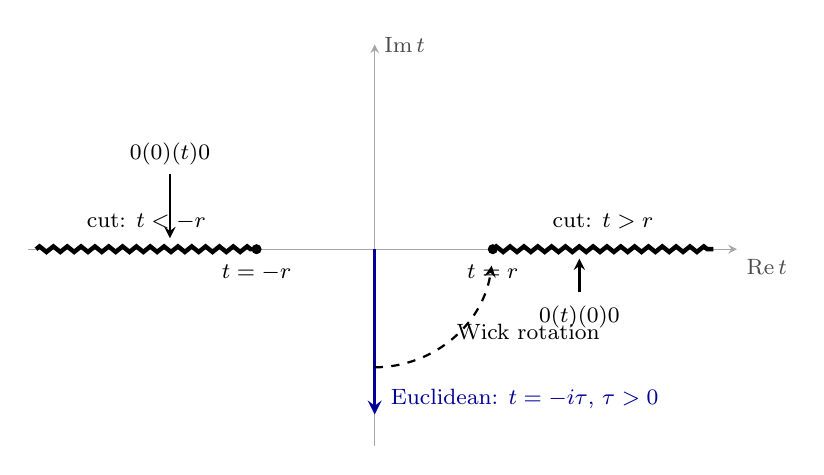
\begin{tikzpicture}[scale=1.0, >=stealth]
  % axes
  \draw[->, gray!70] (-4.4,0) -- (4.6,0) node[below right, black!70] {\footnotesize $\mathrm{Re}\,t$};
  \draw[->, gray!70] (0,-2.5) -- (0,2.6) node[right, black!70] {\footnotesize $\mathrm{Im}\,t$};
  % cuts
  \draw[line width=1.6pt, decorate, decoration={zigzag, segment length=5pt, amplitude=1pt}]
    (1.5,0) -- (4.3,0);
  \draw[line width=1.6pt, decorate, decoration={zigzag, segment length=5pt, amplitude=1pt}]
    (-4.3,0) -- (-1.5,0);
  \node at (2.9,0.35) {\footnotesize cut: $t > r$};
  \node at (-2.9,0.35) {\footnotesize cut: $t < -r$};
  % light cone points
  \filldraw (1.5,0) circle (1.6pt) node[below=2pt] {\footnotesize $t = r$};
  \filldraw (-1.5,0) circle (1.6pt) node[below=2pt] {\footnotesize $t = -r$};
  % Euclidean axis
  \draw[->, very thick, blue!60!black] (0,0) -- (0,-2.1);
  \node[blue!60!black, anchor=west] at (0.08,-1.9) {\footnotesize Euclidean: $t = -i\tau$, $\tau > 0$};
  % Wick rotation path
  \draw[->, thick, dashed] (0,-1.5) arc (-90:-8:1.5);
  \node at (1.95,-1.05) {\footnotesize Wick rotation};
  % boundary values
  \draw[->, thick] (2.6,-0.55) -- (2.6,-0.12);
  \node[anchor=north] at (2.6,-0.6) {\footnotesize $\bra{0}\op(t)\op(0)\ket{0}$};
  \draw[->, thick] (-2.6,0.95) -- (-2.6,0.14);
  \node[anchor=south] at (-2.6,0.95) {\footnotesize $\bra{0}\op(0)\op(t)\ket{0}$};
\end{tikzpicture}
\caption{The complex time plane of the two-point function at fixed spatial
  separation $r$. Positivity of the energy makes the function holomorphic off
  the real axis; singularities reach the real axis only at timelike separation
  $|t| \ge r$. Operator orderings are boundary values from below ($\op(t)$
  acting last) or above; their mismatch across the cuts is the commutator
  \eqref{eq:pauli-jordan}; the Euclidean correlator is the section along the
  negative imaginary axis, reached by Wick rotation $t = e^{-i\theta}|t|$.}
\label{fig:complex-time}
\end{figure}

\begin{exercise}[easy]
\label{exr:massive-wightman}
Repeat Example~\ref{ex:free-scalar-2pt} for the massive free scalar in $d=4$ at
purely spatial separation, and at purely timelike separation. Show that the
Euclidean propagator decays as $e^{-mr}$ at large $r$ (the Yukawa/OZ form, as
anticipated by the correlation-length discussion around
\eqref{eq:ising-correlator}), while at large timelike separation the Wightman
function \emph{oscillates} as $e^{-imt}$ with a power-law envelope. One
analytic function: exponential decay in one direction of the complex plane is
oscillation in the orthogonal one.
\hint{Both behaviors follow from the K\"all\'en--Lehmann representation below
with $\rho(s) = \delta(s - m^2)$; no integral needs to be done exactly. For the
envelope, saddle-point the mode integral.}
\end{exercise}

\begin{exercise}[medium]
\label{exr:retarded}
Define the retarded function $G_R(x) = -i\,\theta(t)\bra{0}[\op(x),
\op(0)]\ket{0}$. Show from the representation \eqref{eq:boundary-value} and its
conjugate that $G_R$ is the boundary value of a function holomorphic when both
$\mathrm{Im}\,t$ \emph{and} the energy variable of its Fourier transform are
continued appropriately: in momentum space, $\tilde G_R(\omega, \mathbf{p})$ is
holomorphic for $\mathrm{Im}\,\omega > 0$. This upper-half-plane analyticity is
the QFT ancestor of the Kramers--Kronig dispersion relations, and the germ of
the dispersive bootstrap methods of Part IX.
\hint{$\theta(t) = \frac{1}{2\pi i}\int d\omega'\, \frac{e^{i\omega'
t}}{\omega' - i\epsilon}$; convolve. Causality (support of $G_R$ in $t \ge 0$)
and analyticity in $\omega$ are Fourier duals of one another.}
\end{exercise}

\subsubsection{The $n$-point dictionary, and how to use it}
\label{sec:npoint-dictionary}

The two-point function fit in one complex plane; the general entry of the
dictionary must be spelled out once, carefully, because every
``Wick rotate the correlator'' step in the rest of these notes silently
invokes it. The statements stack up in four layers, each purchased by one
physical input.\footnote{This subsection states what is proved in
Streater--Wightman, chs.\ 2--3 (the tube theorems and the
Bargmann--Hall--Wightman analysis) and surveyed in Dedushenko
\arxiv{2203.08053}, \S2.1. Our job here is to make the \emph{structure}
usable; the proofs are genuinely analytic and we cite them without
embarrassment.}

\emph{Layer 1 (positive energy): the tube.} Repeating the damping argument of
\eqref{eq:spectral-sum} between each adjacent pair of operators, the
$n$-point Wightman function $W_n(x_1, \dots, x_n)$ --- one fixed ordering ---
extends holomorphically to complex times with \emph{ordered} imaginary parts,
$\mathrm{Im}(t_{k+1} - t_k) < 0$: each successive factor $e^{-iH(t_{k+1} -
t_k)}$ becomes a damping $e^{-H\,|\mathrm{Im}\,\Delta t|}$. (Translation
invariance makes this a statement about the $n-1$ difference variables; with
Lorentz invariance the domain widens in the spatial directions too --- the
``extended tube'' --- but the time story carries all the intuition.)

\emph{Layer 2 (microcausality): the orderings agree where they can.} Distinct
orderings of the same operators are boundary values of \emph{a priori}
different analytic functions. But at spacelike separations the operators
commute, so the functions agree on a real open set --- and holomorphic
functions agreeing on a real open set of their common boundary are
continuations of one another (the \emph{edge-of-the-wedge} theorem, the one
piece of hard analysis this story genuinely needs). All $n!$ orderings thus
assemble into a
\emph{single} analytic function on the union of the permuted domains (the
``permuted extended tube''), and ``the correlator'' becomes a well-defined
single object with many real-time faces --- the $n$-point upgrade of
Figure~\ref{fig:complex-time}.

\emph{Layer 3 (the theorem): Euclidean points are inside.} The classic result
of the axiomatic era is that the purely Euclidean configurations $t_k =
-i\tau_k$, at non-coincident points, lie in the interior of that common
domain. The restriction there --- the Schwinger function $S_n$ --- is
real-analytic and, because the domain is permutation-glued,
\emph{symmetric}: Euclidean correlators have no memory of operator order,
which is why a statistical-mechanics presentation, which never knew about
order, can produce them.

\emph{Layer 4 (the recipe): how to come back.} To recover any Lorentzian
correlator from Euclidean data, give each operator a small positive Euclidean
time offset encoding its place in the desired order and continue:
\begin{equation}
\bra{0}\op_1(t_1)\,\op_2(t_2)\cdots\op_n(t_n)\ket{0}
\;=\;
\lim_{\epsilon_1 > \epsilon_2 > \cdots > \epsilon_n \to 0^+}
S_n\big(\tau_k = \epsilon_k + i t_k\big):
\label{eq:continuation-recipe}
\end{equation}
\emph{operator order = order of the $\epsilon$'s}. Time-ordered correlators
correspond to choosing the $\epsilon$'s in the same order as the real times
themselves --- equivalently, to the uniform rotation $t_k \to (1 -
i\delta)\,t_k$ --- which for two points collapses to the single ``$x^2 +
i\epsilon$'' of Example~\ref{ex:free-scalar-2pt}. This recipe
is worth filing as a reflex --- it is how every Lorentzian statement in these
notes (commutators, response functions, the chaos correlators of Part XI)
will be extracted from Euclidean computations.

The recipe is not hostage to free fields or to perturbation theory, and it
pays to see it act on an interacting correlator at least once.

\begin{eexample}[A Lorentzian correlator of the 2d Ising CFT]
\label{ex:ising-lorentzian}
The critical 2d Ising model has $\langle\sigma(x)\,\sigma(0)\rangle_{\rm E} =
|x|^{-1/4}$ (with $\Delta_\sigma = \tfrac18$ --- a lattice-derivable fact we
import; Part III.4 computes it three ways). What does the \emph{Lorentzian}
critical Ising magnet do? Continue by the recipe: with $x^2_{\rm E} = r^2 +
\tau^2 \to r^2 - (t - i\epsilon)^2$,
\begin{equation}
\bra{0}\sigma(t, r)\,\sigma(0)\ket{0}
= \frac{1}{\big[r^2 - (t - i\epsilon)^2\big]^{1/8}}
= \begin{cases}
\ \big(r^2 - t^2\big)^{-1/8} & \text{spacelike}, \\[4pt]
\ \big(t^2 - r^2\big)^{-1/8}\; e^{-i\pi/8} & \text{timelike, } t > 0,
\end{cases}
\label{eq:ising-wightman}
\end{equation}
since for $t > r$ the argument $r^2 - (t-i\epsilon)^2$ crosses to the
negative reals from the upper side, $(|X| e^{i\pi})^{-1/8} = |X|^{-1/8}
e^{-i\pi/8}$. Three readings. \emph{(i)} At spacelike separation the
correlator is real and order-independent: causality, visible. \emph{(ii)} At
timelike separation it acquires the universal phase $e^{-i\pi \Delta_\sigma}$
--- the operator ordering matters now, the reversed order giving
$e^{+i\pi\Delta_\sigma}$, and the imaginary part
\begin{equation}
\bra{0}[\sigma(t,r), \sigma(0)]\ket{0}
= -\,2i\,\sin\!\big(\tfrac{\pi}{8}\big)\,
\frac{\mathrm{sgn}(t)}{(t^2 - r^2)^{1/8}}
\end{equation}
is a nonvanishing commutator filling the \emph{entire} forward lightcone ---
compare the free massless field \eqref{eq:pauli-jordan}, whose commutator
clung to the cone's surface. An interacting CFT signals at every timelike
separation. \emph{(iii)} The branch-point structure at the lightcone $t = r$,
with its exponent set by an anomalous dimension, is the germ of Lorentzian
CFT technology --- lightcone limits, where the analytic bootstrap of Part
III.3 lives.
\end{eexample}

\begin{exercise}[medium]
\label{exr:ising-spectral}
Check \eqref{eq:ising-wightman} against unitarity: Fourier transform the 2d
Wightman function $W(t, r)$ at $r$-momentum zero and verify the spectral
weight is supported at positive energy and is positive. Then verify
consistency with the K\"all\'en--Lehmann formula \eqref{eq:cft-spectral} of
the next subsection at $d = 2$, $\Delta = \frac18$.
\hint{It is easiest to trust the general theorem and check the phase: the
positivity computation is the $d=2$ case of Exercise~\ref{exr:cft-spectral}.}
\end{exercise}

\subsubsection{The spectral representation, and theories without particles}
\label{sec:kallen-lehmann}

The two-point function earns one more pass, because in an interacting theory
it carries a complete, presentation-independent record of the spectrum. Insert
states organized by total momentum in \eqref{eq:spectral-sum}: Poincar\'e
invariance forces the matrix elements to depend only on the invariant mass, and
the two-point function of any Hermitian scalar operator collapses to a
\emph{one-dimensional} integral over free propagators. In the Euclidean form,
which is the cleanest,
\begin{equation}
\langle \op(x)\, \op(0) \rangle_{\rm E}
= \int_0^\infty ds \; \rho(s)\, G_{\rm free}(x; s),
\qquad
\tilde G(p) = \int_0^\infty ds\; \frac{\rho(s)}{p^2 + s},
\label{eq:kallen-lehmann}
\end{equation}
where $G_{\rm free}(x;s)$ is the free Euclidean propagator of mass$^2$ $s$, and
the \vocab{spectral density}
\begin{equation}
\rho(s) \;\propto\; \sum_n \big|\bra{0}\op(0)\ket{n}\big|^2\,
\delta\big(s - m_n^2\big) \;\ge\; 0
\label{eq:spectral-density}
\end{equation}
is manifestly nonnegative in a unitary theory: it is a sum of squared
amplitudes for $\op$ to create states out of the vacuum. This is the
\vocab{K\"all\'en--Lehmann representation}. Analytically, \eqref{eq:kallen-lehmann}
says the momentum-space two-point function is a Stieltjes transform: holomorphic
in the cut $p^2$ plane, with all its singularities on the negative real axis
$p^2 = -s$ (the Lorentzian on-shell region, $p^2 = -m^2$ in mostly-plus), and
with $\rho$ recoverable as the discontinuity across the cut. Everything we said
about complex time in the previous subsection has become, after Fourier
transformation, a statement about complex momentum.

The representation turns qualitative questions about the spectrum into
questions about the \emph{shape} of $\rho$, answerable by inspecting
correlators alone:

\begin{itemize}
\item \emph{A gapped theory with a stable particle}: $\rho(s) = Z\,\delta(s -
m^2) + (\text{continuum starting at } s \ge (2m)^2)$. The isolated
$\delta$-function is the particle; the gap between it and the multiparticle
continuum is what makes asymptotic states, and hence an S-matrix, exist.
\item \emph{The free massless field}: $\rho(s) = \delta(s)$, one massless
particle and nothing else.
\item \emph{A conformal field theory}: power-law correlators force a power-law
density. For $\langle\op\op\rangle_{\rm E} = 1/x^{2\Delta}$ in $d$ dimensions,
Fourier transformation gives $\tilde G(p) \propto (p^2)^{\Delta - d/2}$ and
\begin{equation}
\rho(s) \;=\; \frac{\pi^{d/2}\, 2^{\,d - 2\Delta}}{\Gamma(\Delta)\,
\Gamma\!\big(\Delta - \tfrac{d}{2} + 1\big)} \; s^{\,\Delta - d/2},
\label{eq:cft-spectral}
\end{equation}
a featureless continuum from $s = 0$ to infinity: no $\delta$-function, no gap,
no threshold (Exercise~\ref{exr:cft-spectral}). This makes precise the claim of
chapter I.1 that a CFT has no particles. There is no state for an asymptotic
wavepacket to converge to, hence no S-matrix; the correlators are not a
stepping stone to the observables --- they \emph{are} the
observables.\footnote{This point, with the same computation, opens Rychkov's
EPFL lectures \arxiv{1601.05000}, \S1.3.1. A dimension close to a free value,
$\Delta = \frac{d-2}{2} + \gamma$ with $\gamma$ small, gives $\rho \sim
s^{\gamma - 1}$: a free particle's $\delta$-function ``melted'' into a sharp
but integrable peak --- the right mental image for an almost-free fixed point
like Banks--Zaks.}
\end{itemize}

And positivity of $\rho$ has teeth. The prefactor in \eqref{eq:cft-spectral}
changes sign when $\Gamma(\Delta - \frac d2 + 1)$ does: for the power law
$1/x^{2\Delta}$ to be the two-point function of \emph{any} operator in a
unitary theory requires
\begin{equation}
\Delta \;\ge\; \frac{d-2}{2},
\label{eq:scalar-unitarity-bound}
\end{equation}
with equality forcing $\rho \to \delta(s)$ --- the free field. This is the
scalar \vocab{unitarity bound}, here derived purely from the Lorentzian
spectral representation, before conformal symmetry has even entered the
chapter. (Part III.1 re-derives it, together with its spin-$\ell$ siblings,
from radial quantization, where it generalizes more easily.) We will reuse both
the bound and the computation behind it when we build the generalized free
field in Example~\ref{ex:gff}.

\begin{exercise}[classic]
\label{exr:cft-spectral}
Derive \eqref{eq:cft-spectral}. First establish the Fourier transform
$\int d^dx \, e^{-ip\cdot x} (x^2)^{-\Delta} = \pi^{d/2}\, 2^{d - 2\Delta}\,
\frac{\Gamma(d/2 - \Delta)}{\Gamma(\Delta)}\, (p^2)^{\Delta - d/2}$ (valid by
analytic continuation in $\Delta$), then extract the spectral density as the
discontinuity of the Stieltjes transform \eqref{eq:kallen-lehmann}, $\rho(s) =
\frac{1}{\pi}\,\mathrm{Im}\,\tilde G(p^2 = -s - i0)$, and use the reflection
formula $\Gamma(z)\Gamma(1-z) = \pi/\sin \pi z$ to reach the quoted form.
Verify: (a) $\rho \ge 0$ iff $\Delta \ge \frac{d-2}{2}$ (for $\Delta$ below the
free value the would-be density oscillates in sign); (b) as $\Delta \to
\frac{d-2}{2}$, $\rho(s) \to \delta(s)$ in the distributional sense.
\hint{For the Fourier transform, use the Schwinger parametrization $(x^2)^{-\Delta}
= \frac{1}{\Gamma(\Delta)}\int_0^\infty du\, u^{\Delta-1} e^{-u x^2}$ and do
the Gaussian integral. For (b), note $s^{\gamma-1}/\Gamma(\gamma) \to
\delta(s)$ as $\gamma \to 0^+$ on test functions, after checking the overall
normalization.}
\answ{The sign of $\rho$ is the sign of $1/\Gamma(\Delta - \frac d2 + 1)$,
positive for $\Delta > \frac d2 - 1$, and the limit (b) is the statement that
the free massless particle is the boundary case of the conformal continuum.}
\end{exercise}

\begin{reemark}[Correlators are distributions; this matters less than you fear]
\label{rem:distributions}
At coincident points correlators blow up --- $1/x^{2\Delta}$ is not a function
at $x = 0$ --- and the axiomatic tradition correspondingly treats fields as
operator-valued \emph{distributions}, to be smeared with test functions before
they act on the Hilbert space. The Wightman axioms (chapter I.1, \S6) make
temperedness an axiom; theories with very fast-growing spectra can violate it
and require finer test-function classes. In these notes we work at non-coincident
points, where everything is real-analytic, and treat the short-distance
behavior not as an analytic nuisance but as the \emph{subject}: the operator
product expansion of Section~\ref{sec:ope} is exactly the statement that the
coincident-point singularity is structured, computable, and --- in a CFT ---
the generating structure of the whole theory.
\end{reemark}

% =====================================================================
\subsection{Reflection positivity: how correlators become a theory}
\label{sec:reflection-positivity}

The previous section moved in one direction: given a quantum theory ---
Hilbert space, positive Hamiltonian, operators --- we produced Euclidean
correlators and located them inside an analytic structure. But the working
direction of modern physics is the reverse. A lattice model, a Euclidean path
integral, a set of bootstrap data: each hands you Schwinger functions and
nothing else. Nobody hands you a Hilbert space. So the honest question --- and
it is the central question of this section --- is: \emph{which} sets of
Euclidean correlation functions are the Euclidean section of a genuine quantum
theory? Statistical averages are cheap; quantum mechanics, with its positive
probabilities and unitary evolution, is not. Something about the Euclidean data
must encode positivity, and whatever it is must be checkable without ever
leaving Euclidean signature.

The answer is a single condition with a mirror in it. To find it, run the
quantum-mechanical construction of states backwards. In a Lorentzian theory we
build states by acting on the vacuum; in the Euclidean section, acting on the
vacuum at negative Euclidean time and evolving to $\tau = 0$ means: a state is
\emph{a collection of operator insertions in the lower half-space} $\tau < 0$.
Call such a collection $F$ --- finitely many operators at points $x_1, \dots,
x_k$ with $\tau_i < 0$, or any linear combination of such. Its conjugate state,
by the continuation rule \eqref{eq:boundary-value} read backwards, is the
\emph{time-reflected, complex-conjugated} collection $\Theta F$, living in the
upper half-space: Euclidean time reflection $\theta(\tau, \mathbf{x}) = (-\tau,
\mathbf{x})$ is what Hermitian conjugation looks like after Wick
rotation.\footnote{One line of algebra: Euclidean Heisenberg evolution
$\op(\tau, \mathbf{x}) = e^{H\tau}\op(0,\mathbf{x})\,e^{-H\tau}$ is \emph{not}
unitary, so for a scalar Hermitian at $\tau = 0$,
$\op(\tau, \mathbf{x})^\dagger = e^{-H\tau}\op(0,\mathbf{x})\,e^{H\tau} =
\op(-\tau, \mathbf{x})$: the conjugate lives at the mirror point. Operators with
spin pick up a reflection acting on their indices; see Simmons-Duffin
\arxiv{1602.07982}, \S7.1, whose treatment we follow, and
Appendix~\ref{app:conventions}.} The norm of the state is then a correlator with
mirror-symmetric insertions,
\begin{equation}
\big\| \,F\, \big\|^2 \;=\; \big\langle\, (\Theta F)\; F \,\big\rangle ,
\label{eq:rp-norm}
\end{equation}
and quantum mechanics demands it be nonnegative. That is the condition.

\begin{ddefinition}[Reflection positivity]
\label{def:reflection-positivity}
A collection of Schwinger functions is \vocab{reflection positive} with respect
to a hyperplane (say $\tau = 0$) if for every finite linear combination $F =
\sum_\alpha c_\alpha\, \op_{1}(x^\alpha_1)\cdots\op_{k_\alpha}(x^\alpha_{k_\alpha})$
of insertions supported at $\tau < 0$,
\begin{equation}
\sum_{\alpha,\beta} \bar c_\alpha\, c_\beta \,
\big\langle\, \theta\big[\op_{1}(x^\alpha_1)\cdots\big]^{*} \;
\op_{1}(x^\beta_1)\cdots \,\big\rangle \;\ge\; 0,
\label{eq:rp-def}
\end{equation}
where $\theta$ reflects all insertion points through the hyperplane and
conjugates coefficients. Reflection positivity is the Euclidean avatar of
unitarity, and we will use the two words interchangeably once the dictionary is
established.
\end{ddefinition}

\noin Two remarks before we test the definition on a lattice. First, the
condition involves a \emph{choice} of hyperplane, but Euclidean invariance of
the correlators promotes positivity across one plane to positivity across all
of them --- a freedom that looks innocent and is not: making radically
different choices of ``cut'' is precisely how radial quantization will fall out
of this machinery in Section~\ref{sec:ope}. Second, the definition never
mentions a Hilbert space; it is a property of a list of functions, checkable
configuration by configuration on a lattice. That is its entire value.

\begin{eexample}[Reflection positivity on the lattice, by transfer matrix]
\label{ex:lattice-rp}
Return to the Ising chain of Example~\ref{ex:ising-chain}: spins $s_i = \pm1$,
weight $\prod_i e^{J s_i s_{i+1}}$, and now take the chain infinite (or long,
with free ends --- the boundary will not matter). Reflect through the
\emph{bond} between sites $0$ and $1$: $\theta(i) = 1 - i$ maps the right half
$\{i \ge 1\}$ onto the left half $\{i \le 0\}$. Let $F$ be any real function of
the spins on the right half. Reflection positivity asks for $\langle
(\theta F)\, F\rangle \ge 0$.

Sum first over the spins strictly inside each half, holding the boundary spins
fixed. All the dependence collapses into a single function of one spin,
\begin{equation}
v_F(s_1) \;=\; \sum_{\{s_i\}_{i \ge 2}} F(s_1, s_2, \dots)
\prod_{i \ge 1} e^{J s_i s_{i+1}},
\end{equation}
and, by the mirror symmetry of the construction, the left half produces the
\emph{same} function of $s_0$. The full average is then a $2\times2$ quadratic
form threaded by the one bond that crosses the mirror:
\begin{equation}
\langle (\theta F)\, F \rangle \;\propto\; \sum_{s_0, s_1}
v_F(s_0) \, e^{J s_0 s_1} \, v_F(s_1)
\;=\; v_F^{\,T}\, T \, v_F ,
\qquad
T = \begin{pmatrix} e^J & e^{-J} \\ e^{-J} & e^{J}\end{pmatrix}.
\label{eq:rp-transfer}
\end{equation}
This is nonnegative for every $F$ if and only if the bond matrix $T$ ---
the transfer matrix of Example~\ref{ex:ising-chain} --- is \emph{positive
definite}. Its eigenvalues are $2\cosh J$ and $2\sinh J$: both positive for
the ferromagnet $J > 0$. The Ising chain is reflection positive, and the proof
is two lines once the transfer matrix exists.

The example repays a second look, because each ingredient is a general lesson
in miniature.
\emph{(i)} What reflection positivity actually delivered is the statement that
$T$ is a positive operator, $T = e^{-aH}$ for a Hermitian $H$ bounded below
(here $H = -\frac1a \log T$, finite because both eigenvalues are positive). In
chapter I.1 we \emph{matched} $T \approx e^{-aH}$ in the continuum limit as a
computational device; reflection positivity is the structural reason a
Hamiltonian had to be there. A statistical weight whose mirror-symmetric
averages are positive contains a quantum theory, and the Hamiltonian is the
logarithm of the weight.
\emph{(ii)} The positivity was not automatic. For the antiferromagnet $J < 0$
the bond matrix has a negative eigenvalue and bond-reflection positivity
\emph{fails} --- though reflection through a \emph{site} ($\theta(i) = -i$,
which fixes site $0$) still works: summing out everything except the mirror
spin gives $\langle(\theta F) F\rangle \propto \sum_{s_0} u_F(s_0)^2 \ge 0$
identically. Which reflections are positive is a real, useful invariant of a
lattice model (site- vs.\ bond-centered reflections are the germ of the
chessboard estimates of rigorous statistical mechanics), and on the bipartite
lattice the antiferromagnet is rescued by a sublattice flip --- a baby example
of positivity holding only after a dressing.
\emph{(iii)} Complex couplings break everything: for the chain in an imaginary
magnetic field, $e^{h s_i}$ with $h$ imaginary, the weight is not positive,
reflection positivity fails, and yet the model has a perfectly sharp critical
point --- the Lee--Yang edge singularity, governed by a \emph{non-unitary}
conformal field theory (Exercise~\ref{exr:lee-yang}). Reflection positivity is
a genuine axiom, not a formality: nature's statistical-mechanics corner is
populated by theories that violate it and are interesting for that very reason.
\end{eexample}

\begin{exercise}[easy]
\label{exr:rp-2d-ising}
Extend the bond-reflection argument to the two-dimensional Ising model on a
rectangular lattice (reflect through a line of bonds; the boundary data is now
a whole column of spins $\mathbf{a} = (s_{1,j})_j$). Show $\langle (\theta F) F
\rangle = \sum_{\mathbf{a}, \mathbf{b}} v_F(\mathbf{a})\, K(\mathbf{a}, \mathbf{b})\, v_F(\mathbf{b})$
with $K(\mathbf{a}, \mathbf{b}) = \prod_j e^{J a_j b_j}$, and prove $K$ is a positive
matrix.
\hint{$e^{J a b} = \cosh J + ab \sinh J$ for $a, b = \pm 1$, so $K$ is a tensor
product of $2\times2$ positive matrices when $J > 0$.}
\end{exercise}

\begin{exercise}[thinker]
\label{exr:lee-yang}
(Lee--Yang, or life without positivity.) Consider the Ising chain in a purely
imaginary field, weight $\exp[\sum_i (J s_i s_{i+1} + i h_{\rm I} s_i)]$ with
$h_{\rm I}$ real. (a) Show the transfer matrix is no longer Hermitian, find
where its eigenvalues collide as $h_{\rm I}$ grows at fixed $J$, and conclude
the free energy has a singularity at real $h_{\rm I}$ --- the Lee--Yang edge,
which in $d \ge 2$ becomes a genuine critical point. (b) Exactly which step of
Example~\ref{ex:lattice-rp} fails? (c) The corresponding CFT (Fisher; in 2d the
minimal model $\mathcal{M}(2,5)$, cf.\ Part III.4) has an operator with
$\Delta < 0$, flatly violating \eqref{eq:scalar-unitarity-bound}. Reconcile:
which physical statements of this chapter survive without unitarity
(analyticity? OPE?) and which do not (norms? bounds?).
\hint{For (a): eigenvalue collision of a non-Hermitian $2\times2$ matrix means
a square-root branch point --- the edge exponent in $d=1$. For (c): analytic
continuation needed only $H$ bounded below in some sector; positivity of norms
is what fails.}
\end{exercise}

\subsubsection{The reconstruction theorem, sketched honestly}
\label{sec:os-reconstruction}

Reflection positivity is necessary for a quantum interpretation. The
remarkable fact --- the central structural theorem of axiomatic QFT, and the
license for everything these notes do in Euclidean signature --- is that
together with a short list of statistical-mechanics properties it is
\emph{sufficient}: the entire quantum theory can be excavated from the
Schwinger functions. The hard analysis is due to Osterwalder and Schrader and
we will not reproduce it, but the \emph{construction} at its heart is short,
beautiful, and worth doing for real --- it is the construction we will reuse,
with spheres in place of planes, to prove OPE convergence. We follow the
blueprint already visible in the lattice example.

Suppose, then, we are given Schwinger functions $S_n$ for some set of local
operators, satisfying: Euclidean covariance; symmetry under permutations;
reflection positivity \eqref{eq:rp-def}; cluster decomposition; and a
temperedness/growth condition on their short-distance singularities (this last
is the fine print --- see the Note below --- and we suppress it until it
matters). Construct:

\emph{Step 1: the pre-Hilbert space.} Let $V$ be the complex vector space of
formal finite linear combinations of insertion-collections in the lower half
space, $F = \sum_\alpha c_\alpha\, \op(x_1^\alpha)\cdots\op(x^\alpha_{k_\alpha})$,
all $\tau$'s negative. Define a sesquilinear form on $V$ using only the given
correlators:
\begin{equation}
\langle F, G\rangle \;\equiv\; \big\langle (\Theta F)\, G \big\rangle
\;=\; \sum_{\alpha\beta} \bar c_\alpha c_\beta\,
S_{k_\alpha + k_\beta}\big(\theta x^\alpha_1, \dots;\; x^\beta_1, \dots\big).
\label{eq:os-inner-product}
\end{equation}
Reflection positivity says precisely that this form is positive semidefinite.

\emph{Step 2: quotient and complete.} The null vectors $N = \{F : \langle F,
F\rangle = 0\}$ form a subspace (Cauchy--Schwarz, which positive semidefinite
forms obey), and on the quotient $V/N$ the form is a genuine inner product.
Complete it:
\begin{equation}
\mathcal{H} \;\equiv\; \overline{V / N}.
\end{equation}
This is \emph{the} Hilbert space of the theory --- not a Hilbert space
postulated alongside the correlators, but one manufactured from them. The
vacuum is the class of the empty insertion, $\ket{0} = [\,\mathbf{1}\,]$, with
$\braket{0}{0} = S_0 = 1$. (The quotient is doing real physics: on the lattice,
many different right-half configurations of insertions produce the same state
on the mirror --- $V/N$ \emph{is} the boundary Hilbert space $\complex^2$ of
the chain, as Exercise~\ref{exr:os-chain} makes explicit. Gauge theory will
make the quotient earn its keep even more visibly, with Gauss-law violating
configurations becoming null.)

\emph{Step 3: the Hamiltonian.} Euclidean time translation acts on insertions:
$(T_\sigma F)$ shifts every insertion by $\tau \to \tau - \sigma$, $\sigma > 0$,
staying in the lower half-space. The form \eqref{eq:os-inner-product} is
reflection-symmetric, so $T_\sigma$ is a symmetric operator on $V/N$, and a
two-line Cauchy--Schwarz induction (Exercise~\ref{exr:contraction}) shows it is
a \emph{contraction}: $\|T_\sigma F\| \le \|F\|$. A symmetric contraction
semigroup has a self-adjoint, nonnegative generator:
\begin{equation}
T_\sigma = e^{-\sigma H}, \qquad H = H^\dagger \ge 0 .
\label{eq:os-hamiltonian}
\end{equation}
Pause on what just happened. In Section~\ref{sec:analytic-structure},
positivity of the energy was the \emph{input} and Euclidean analyticity the
output. Here the direction is reversed: reflection positivity of statistical
averages \emph{produced} a positive Hamiltonian. The two positivities are the
same fact seen from the two sides of the Wick rotation --- this is the precise
sense in which Euclidean field theory is not a trick but an equivalent
formulation.

\emph{Step 4: operators, and back to Wightman.} A local operator at $\tau = 0$
is the limit of insertions approaching the mirror from below; smeared
suitably, these become densely defined operators on $\mathcal{H}$. The
remaining Euclidean symmetries come along: spatial translations and rotations
act on insertions and descend to unitaries on $\mathcal{H}$; the rotations that
mix Euclidean time with space do \emph{not} descend to unitaries --- they
become, upon the analytic continuation now justified by
\eqref{eq:os-hamiltonian} and the spectral theorem, the \emph{boosts} of a
unitary representation of the Poincar\'e group, and the analytically continued
correlators of the reconstructed operators are Wightman functions satisfying
the full set of Wightman axioms. This last step --- controlling the
continuation of $n$-point functions, not just of the semigroup --- is where the
real work and the growth condition live, and is what we cite rather than
derive.\footnote{Osterwalder--Schrader, \emph{Axioms for Euclidean Green's
functions} I, Comm.\ Math.\ Phys.\ \textbf{31} (1973) 83, and II, \textbf{42}
(1975) 281. The survey of this and the neighboring axiom systems
(Glimm--Jaffe's, Nelson's, with their respective reconstruction theorems) is
Dedushenko \arxiv{2203.08053}, \S2.1, which this subsection compresses.}

\begin{ttheorem}[Osterwalder--Schrader reconstruction]
\label{thm:os}
Schwinger functions satisfying Euclidean covariance, permutation symmetry,
reflection positivity, cluster decomposition, and a linear-growth temperedness
condition are the Euclidean continuation of a unique unitary quantum field
theory satisfying the Wightman axioms --- with Hilbert space, vacuum, positive
Hamiltonian, Poincar\'e representation, and field operators all constructed
from the Schwinger functions as in Steps 1--4. Cluster decomposition of $S_n$
becomes uniqueness of the vacuum.
\end{ttheorem}

\begin{nnote}
The growth condition is not decoration. Osterwalder and Schrader's first paper
claimed reconstruction without it; the proof contained a gap, and the
linear-growth hypothesis of their second paper (each $S_n$ bounded by
factorially many derivatives in a controlled way) is what makes the
continuation of all $n$-point functions converge. There exist sets of
Schwinger functions satisfying every other axiom whose continuation fails ---
positivity across planes alone does not see fast enough growth in $n$. For the
theories in these notes the condition is verified wherever rigorous
constructions exist ($d = 2, 3$ scalar theories, cf.\ chapter I.1's
constructive inventory), and for CFTs the OPE of the next section supplies a
far stronger handle on coincident-point growth. We flag it once, here, and
trust it silently hereafter.
\end{nnote}

\begin{iidea}[Correlators are the theory]
\label{idea:correlators-are-theory}
With reflection positivity, the slogan of chapter I.1 becomes a construction:
the Hilbert space is built from Euclidean correlators (insertions modulo null
configurations), the Hamiltonian is the generator of Euclidean time shifts
acting on them, and the field operators are insertions approaching the cut.
Nothing else needs to be given. Whoever specifies consistent correlators ---
a lattice at criticality, a bootstrap dataset $\{\Delta_i, c_{ijk}\}$, a
mythical path integral --- has specified a complete quantum theory, whether or
not any Lagrangian is anywhere in sight.
\end{iidea}

There is one loose thread, deliberately left hanging, and it deserves to be
tied into a principle. Look back at what the construction actually used: not
the plane as such, but a \emph{reflection}. The working parts were an
involution $\theta$ exchanging two halves of Euclidean space, positivity of
the correlators on mirror-symmetric configurations, and a family of
translates of the mirror to evolve along; the plane $\tau = 0$ appeared only
as the mirror's fixed locus. Stated invariantly: \emph{a quantization of
Euclidean data is a choice of reflection-with-positivity together with a
compatible foliation}. Parallel planes are one such choice --- and since
Euclidean correlators have no preferred time, every hyperplane gives one, all
unitarily equivalent. The productive question writes itself: are there
reflections of a genuinely different shape, quantizing the \emph{same}
correlators in different and useful coordinates? For conformal theories the
answer is the single most consequential move in the subject, and it is
Section~\ref{sec:ope}'s; but first, a short interlude on a question the
reconstruction theorem begs.

\begin{exercise}[medium]
\label{exr:contraction}
Prove the contraction property in Step 3: for any $F$ in the lower half-space
and $T_\sigma$ the shift, show $\|T_\sigma F\|^2 = \langle F, T_{2\sigma}
F\rangle \le \|F\| \, \|T_{2\sigma}F\|$, iterate to $\|T_\sigma F\| \le \|F\|^{1 - 2^{-n}}
\|T_{2^n \sigma}F\|^{2^{-n}}$, and use the temperedness of correlators (no
blow-up of $\|T_\sigma F\|$ as $\sigma \to \infty$, by clustering) to conclude
$\|T_\sigma F\| \le \|F\|$. Where did reflection symmetry of the inner product
enter?
\hint{$\langle T_\sigma F, T_\sigma F\rangle = \langle F, T_{2\sigma}F\rangle$
uses $\Theta T_\sigma = T_{-\sigma} \Theta$: shifting both halves away from the
mirror by $\sigma$ is one shift by $2\sigma$ across it.}
\end{exercise}

\begin{exercise}[classic]
\label{exr:os-chain}
(Reconstruction, executed completely.) Run Steps 1--3 on the Ising chain.
Take as input \emph{only} the correlators $\langle s_{i_1}\cdots
s_{i_n}\rangle$ computed in Example~\ref{ex:ising-chain}. Show: (a) the space
of right-half insertion collections, modulo null vectors, is exactly
two-dimensional (every collection of insertions at sites $\ge 1$ is equivalent,
as a state, to a combination of ``nothing'' and ``one spin at site 1''); (b)
the inner product reproduces $\complex^2$ with the transfer-matrix inner
product; (c) the reconstructed $e^{-aH}$ is $T/\lambda_+$ (normalizing the
ground-state energy to zero), with $H$ matching the continuum limit
\eqref{eq:ising-continuum} as $a \to 0$. This is the smallest nontrivial
instance of Theorem~\ref{thm:os}, with every analytic subtlety absent.
\hint{For (a): on the lattice, $v_F$ in \eqref{eq:rp-transfer} is the state;
two functions of one Ising spin span a two-dimensional space. Null vectors are
collections with $v_F = 0$.}
\end{exercise}

% =====================================================================
\subsection{Interlude: which Euclidean backgrounds are allowed?}
\label{sec:ks-interlude}

The reconstruction theorem connects flat Euclidean space to flat Minkowski
space, and for this chapter that is nearly all we need. But the inventory of
chapter I.1 assigns partition functions and correlators to \emph{curved}
backgrounds too, and there the phrase ``Wick rotation'' quietly loses its
meaning: a generic curved spacetime has no preferred time coordinate to rotate,
and a generic smooth manifold has no canonical complexification for $t$ to
wander into. Since these notes will spend their lives on spheres, tori, and
cylinders --- starting two sections from now, when a sphere becomes a Hilbert
space --- it is worth knowing the modern answer, due to Kontsevich and Segal,
to the question: \emph{on which backgrounds should a QFT's Euclidean data be
expected to exist at all?} Their move is characteristically simple: do not
complexify time --- complexify the \emph{metric}.\footnote{Kontsevich--Segal
\arxiv{2105.10161}, \S2, which this section follows including its notation.
The idea: the archetype of every path integral is the oscillatory Gaussian
$\int e^{\frac i2 x^T A x}$, which one \emph{defines} as a boundary value from
the domain of complex symmetric $A$ with positive-definite imaginary part,
where the integral honestly converges. The space of complex metrics below is
the field-theory version of that domain; Lorentzian signature will sit on its
boundary exactly as the real $A$'s sit on the boundary of the Siegel
half-plane.}

Allow, then, the metric at each point to be a complex-valued quadratic form
$g = \sum_i \lambda_i\, dy_i^2$ (every complex symmetric form can be brought to
this shape in a real basis; the $\lambda_i$ are nonzero complex numbers).
Which $\lambda_i$ should be admitted? The criterion must be that the Euclidean
weight \emph{damps}: every reasonable quadratic action should have positive
real part, so that the path integral has a chance to converge. Run this
requirement through the simplest matter content. For a free scalar on the
(constant, diagonal) complex metric,
\begin{equation}
S[\phi] = \frac{1}{2}\int d^dy \;(\det g)^{1/2}
\left[\, \sum_i \frac{1}{\lambda_i}\,(\partial_i \phi)^2 + m^2 \phi^2 \right],
\qquad
(\det g)^{1/2} = \prod_i \lambda_i^{1/2},
\label{eq:ks-scalar-action}
\end{equation}
with the square root taken with positive real part. Convergence of $\int
\de\phi\, e^{-S}$ requires the coefficient of each quadratic term to have
positive real part:
\begin{equation}
\Big|\arg \frac{\prod_j \lambda_j^{1/2}}{\lambda_i}\Big| < \frac\pi2
\quad\text{for each } i,
\qquad\text{i.e.}\qquad
\Big|\, \tfrac12 \textstyle\sum_{j \ne i} \arg\lambda_j - \tfrac12
\arg\lambda_i \Big| < \frac\pi2 .
\label{eq:ks-scalar-condition}
\end{equation}
A scalar is the $p = 0$ member of a family every QFT bookkeeper must admit:
$p$-form gauge fields, with actions $\int F \wedge \star F$ whose quadratic
forms carry coefficients $(\prod_j \lambda_j^{1/2}) / (\lambda_{i_1} \cdots
\lambda_{i_{p+1}})$ for each index set. Demanding positive real part for
\emph{all} $p$ and all index sets, the worst case is the index set that
collects all the $\lambda$'s whose arguments share a sign, and the family of
conditions collapses into a single clean inequality (Exercise~\ref{exr:ks-worst}):

\begin{ttheorem}[Allowable complex metrics (Kontsevich--Segal)]
\label{thm:ks}
A complex metric $g = \sum_i \lambda_i dy_i^2$ admits convergent quadratic
actions for $p$-form fields of every degree if and only if
\begin{equation}
\sum_{i=1}^{d} \big|\arg \lambda_i \big| \;<\; \pi .
\label{eq:ks-criterion}
\end{equation}
A QFT's partition functions and correlators are expected to extend
holomorphically over the space of metrics satisfying \eqref{eq:ks-criterion}
pointwise --- and no further.
\end{ttheorem}

\noin Now stand back and look at what the inequality says about
\emph{signature}. For a \emph{real} metric every $\arg\lambda_i$ is $0$ or
$\pi$. Euclidean metrics (all arguments $0$) sit comfortably inside the domain.
A real metric with one negative eigenvalue --- Lorentzian signature ---
saturates the bound, $\sum|\arg\lambda_i| = \pi$: it lies exactly \emph{on the
boundary} of the allowed domain, reachable as a limit of allowable metrics but
not itself allowable. And a real metric with two or more time directions
overshoots, $\sum|\arg\lambda_i| \ge 2\pi$: it cannot be reached from the
Euclidean domain at all. Among all real signatures, precisely the Riemannian
and the Lorentzian ones touch the world where path integrals converge. The
old question ``why is the time direction special?'' acquires a sharp,
QFT-internal answer: \emph{Lorentzian spacetimes are the boundary points of the
domain of convergent Euclidean field theory} --- the place where damping
degenerates into pure oscillation, just as $e^{iHt}$ is the boundary behavior
of $e^{-H\tau}$.\footnote{Kontsevich--Segal sharpen ``boundary'' to
\emph{Shilov boundary} --- the minimal set controlling maxima of holomorphic
functions, on which the time-oriented Lorentzian metrics sit --- and prove
the criterion guarantees convergence not just of actions but of the
$p$-form partition functions themselves on tori. We take up that refinement,
the application to curved backgrounds, and the Segal-style gluing axioms it
serves, in chapter I.4.}

Our flat-space Wick rotation now embeds as the simplest possible path through
the domain. Rotate the time coordinate by phase, $t = e^{-i\theta}\,\tau$: the
metric component along it is $\lambda_t = e^{-2i\theta}$, all other
$\lambda$'s real positive, so $\sum_i|\arg\lambda_i| = 2\theta$, which sweeps
from $0$ (Euclidean) to $\pi$ (Lorentzian) as $\theta\colon 0 \to \pi/2$ ---
always allowable until the endpoint. The $i\epsilon$ prescriptions of
Section~\ref{sec:analytic-structure}, and the dashed quarter-circle in
Figure~\ref{fig:complex-time}, are this path seen by the correlators: the
small imaginary part is the last trace of the damping domain, kept alive until
the boundary value is taken.

\begin{ppreview}[Where this goes]
Chapter I.4 uses allowability to answer ``on which complex backgrounds does
the inventory make sense?'' --- including the cylinder-with-complexified-time
geometries that interpolate between partition functions and return amplitudes,
and the curved-space version of the state--operator map. Beyond these notes'
Part I: the criterion has become a working tool in quantum gravity and
cosmology (which complex saddles of the gravitational path integral are
admissible), precisely because it is a statement about QFT on a background,
needing no theory of the metric's own dynamics.
\end{ppreview}

\begin{exercise}[medium]
\label{exr:ks-worst}
Prove Theorem~\ref{thm:ks} from the $p$-form conditions. The coefficient for
the $(p+1)$-form field strength along directions $I = \{i_1 < \cdots <
i_{p+1}\}$ has argument $\frac12\sum_j \arg\lambda_j - \sum_{i \in I}
\arg\lambda_i$. Show that as $I$ ranges over all subsets (all $p$), the
supremum of the absolute value of this quantity is exactly
$\frac12\sum_j|\arg\lambda_j|$, attained by taking $I$ to be the set of all
indices with $\arg \lambda_i > 0$ (or its complement). Conclude that all
coefficients have positive real part iff \eqref{eq:ks-criterion} holds.
\hint{Adding to $I$ an index with $\arg\lambda_i > 0$ decreases the running
total by $\arg\lambda_i$; starting from $\frac12\sum_j \arg \lambda_j$, the
extremes over subsets are $\pm\frac12 \sum_j |\arg\lambda_j|$.}
\end{exercise}

\begin{exercise}[easy]
\label{exr:complex-beta}
(Allowability in $d=1$ is something you already know.) The partition function
of the particle on a circle, Example~\ref{ex:particle-circle}, was $Z(\beta) =
\tr\, e^{-\beta H}$. For which complex $\beta$ does the trace converge?
Interpret the answer via Theorem~\ref{thm:ks} for the metric $g = \beta^2
dt^2$ on the circle of unit coordinate length, and identify the boundary
points $\beta = \pm i T$ as the Lorentzian return amplitudes $\tr\,
e^{\mp iHT}$ --- the $d=1$ shadow of ``Lorentzian signature lives on the
boundary of the allowable domain.''
\answ{$\mathrm{Re}\,\beta > 0$, i.e.\ $|\arg \beta| < \pi/2$, i.e.\
$|\arg\lambda| = |2\arg\beta| < \pi$: the KS criterion verbatim.}
\end{exercise}

% =====================================================================
\subsection{The operator product expansion}
\label{sec:ope}

Now for the third debt: structure. The set of all $n$-point functions of all
local operators is not data anyone could ever specify --- it is an infinite
tower of functions of growing numbers of variables, tangled by consistency
conditions. If ``the theory is its correlators'' is to be a usable definition
rather than a shrug, the tower must be generated by something finite, or at
least finitely describable. The generating structure exists, and it is the
\vocab{operator product expansion}: the statement that the product of two
nearby local operators is itself expandable in local operators,
\begin{equation}
\op_1(x)\,\op_2(0) \;=\; \sum_{k} C_{12k}(x)\; \op_k(0),
\label{eq:ope-schematic}
\end{equation}
with c-number coefficient functions $C_{12k}$, valid as an operator equation
--- i.e.\ inside arbitrary correlators, as long as the other insertions keep
their distance. Used iteratively, \eqref{eq:ope-schematic} grinds any
$n$-point function down to a sum of lower-point ones: the tower of correlators
collapses onto knowledge of the OPE coefficients and the two-point functions.
Wilson proposed exactly this in 1969 --- under the name \emph{operator
algebra}, and as a candidate \emph{definition} of a theory, an ambition the
textbooks quietly downgraded\footnote{K.~Wilson, Phys.\ Rev.\ \textbf{179}
(1969) 1499; Kadanoff's contemporaneous operator algebra of the 2d Ising
model, PRL \textbf{23} (1969) 1430, was the statistical-mechanics twin.
Polyakov's 1974 bootstrap manifesto (chapter I.1, crack 3) is this proposal
plus the demand of crossing. The downgraded, asymptotic version became a
precision instrument in QCD --- deep inelastic scattering is organized by it
--- which is part of why its original ambition was forgotten.} --- and the
central fact of this section is that in a conformal field theory the original
ambition was right: the expansion \eqref{eq:ope-schematic} \emph{converges} at
finite separation, with a computable, geometric radius of convergence and an
exponential rate. Not an asymptotic series that happens to work: a convergent
expansion in the same sense as a Fourier series, and for the same reason ---
it \emph{is} an expansion of a Hilbert-space vector in a complete orthogonal
basis. But first we should understand why \emph{any} expansion of the form
\eqref{eq:ope-schematic} should exist, in any local theory, conformal or not
--- because the argument for existence already contains, in embryo, the
argument for convergence.

\subsubsection{Why an OPE at all: integrating out a ball}
\label{sec:ope-ball}

Here is the path-integral argument, which works in any presentation with a
notion of locality and makes no mention of conformal symmetry. Consider a
correlator with two nearby insertions $\op_1(x_1)\,\op_2(x_2)$ and arbitrary
spectators far away. Draw a sphere $S$ of radius $R$ around the close pair,
small enough to exclude every spectator, and compute the path integral in two
stages: first over the field configurations \emph{inside} $S$ with boundary
values $\phi_\partial$ held fixed, then over everything outside. Locality of
the action is what permits the split --- the weight $e^{-S_{\rm E}}$
factorizes across the sphere up to the shared boundary data. The inside
integral,
\begin{equation}
\Psi_{12}\big[\phi_\partial\big] \;=\;
\int_{\phi|_S = \phi_\partial} \de\phi\;
\op_1(x_1)\,\op_2(x_2)\; e^{-S_{\rm E}[\phi]_{\rm inside}},
\label{eq:ball-functional}
\end{equation}
is a functional of the boundary data alone, and it is the \emph{only} place
$x_1$ and $x_2$ appear: as far as the outside world is concerned, the pair of
operators has been replaced by a blob --- a particular boundary functional on
$S$. Now expand the blob in any complete set of boundary functionals, and
choose for that set the functionals generated by \emph{single} insertions at
the center: $\Psi_k[\phi_\partial] = \int \de\phi\;\op_k(0)\, e^{-S_{\rm E}}$.
The expansion coefficients are c-numbers carrying all the $x_1, x_2$
dependence,
\begin{equation}
\Psi_{12} = \sum_k C_{12k}(x_1, x_2)\, \Psi_k
\qquad\Longrightarrow\qquad
\op_1(x_1)\,\op_2(x_2) \;=\; \sum_k C_{12k}(x_1, x_2)\;\op_k(0)
\label{eq:ball-ope}
\end{equation}
inside any correlator whose other insertions stay outside $S$. That is the
OPE, with its domain of validity --- a separating sphere --- already attached
by the derivation. Two operators close together \emph{are} a superposition of
single operators, in precisely the sense that two charges close together are
a multipole expansion: seen from outside, only the total ``moments'' survive,
and the moments of a local theory are its local operators.

What the argument does not deliver is control. ``Expand in a complete set
of boundary functionals'' begs three questions --- complete by what
criterion, in which topology, with what convergence --- and in a generic
massive theory none has a useful answer: the expansion
\eqref{eq:ball-ope} holds only \emph{asymptotically} in the limit $x_1 \to
x_2$, with coefficient functions $C_{12k}$ that depend on all the scales
and must themselves be computed. (This asymptotic version, with logarithms
resummed by the renormalization group, is the OPE of the QCD textbooks: the
organizing principle of deep inelastic scattering, where it earns its keep
order by order without ever being summed.) The missing ingredient is a
\emph{Hilbert space} statement: were the boundary functionals on $S$
organized into a genuine orthogonal basis adapted to the geometry, the
expansion would be exact and convergent by the elementary theory of Hilbert
spaces. Building exactly that structure is what reflection positivity, run
on spheres, does for us in a CFT --- and it is the only ingredient of the
construction that needs conformal symmetry.

\subsubsection{Radial quantization: reconstruction with spheres}
\label{sec:radial-quantization}

Section~\ref{sec:os-reconstruction} ended with a principle: a quantization of
Euclidean correlators is a reflection-with-positivity plus a compatible
foliation, the constant-$\tau$ planes being merely the first instance. Once
the theory is \emph{conformal}, a second instance exists, and it is strictly
superior for studying local operators: take for the mirror the
\vocab{inversion} $x^\mu \to x^\mu/x^2$, whose fixed locus is the unit
sphere, and for the foliation the concentric spheres $S^{d-1}$ that it
preserves --- inversion exchanges their interiors and exteriors exactly as
$\theta$ exchanged the half-spaces.

Run the reconstruction verbatim. A \emph{state} is now a collection of
insertions \emph{inside} the unit sphere, modulo null collections; the Hilbert
space $\mathcal{H}_{S^{d-1}}$ is their completion --- this is item 3 of the
inventory (Definition~\ref{def:inventory}), realized concretely for the
$(d-1)$-sphere. Evolution from sphere to sphere is generated by the
\vocab{dilatation} operator $D$, which plays the role of the Hamiltonian: in a
scale-invariant theory, rescaling $x \to \lambda x$ maps each leaf of the
foliation to another, exactly as time translation slid the planes. Writing $r
= e^{\tau}$, radial evolution is $e^{-\tau D}$, and ``radial time'' $\tau =
\log r$ runs from $-\infty$ (the origin) to $+\infty$ (the point at
infinity).\footnote{Radial quantization conventions follow Simmons-Duffin
\arxiv{1602.07982}, \S\S6--7 (our default for CFT material; see
Appendix~\ref{app:conventions}, which collects the conformal algebra and the
inversion conjugation we use). The one fact this chapter leans on: $P_\mu$
(translations) and $K_\mu$ (special conformal transformations) raise and lower
radial energy, $[D, P_\mu] = P_\mu$ and $[D, K_\mu] = -K_\mu$. We use the
algebra as bookkeeping; its derivation from conformal invariance, and the
representation theory built on it, is chapter III.1's business.} The role
of time reflection $\theta$ --- Hermitian conjugation's Euclidean shadow ---
passes to the inversion, and reflection positivity across planes becomes
\emph{inversion positivity}; this is not a new assumption, because a
conformal transformation conjugates the planar mirror into the spherical one
and carries the one positivity rigorously onto the
other.\footnote{The plane-to-sphere dictionary is a
conformal conjugation: the generator $K_1 + P_1$, whose flow foliates
$\reals^d$ by spheres through two fixed points, is conjugate to $D$ inside the
conformal group, and the corresponding ``N--S quantization'' interpolates
between planar and radial pictures --- see Rychkov \arxiv{1601.05000},
\S3.1.5, and the original treatment of L\"uscher--Mack. Conjugation in radial
quantization is $\op(x)^\dagger = x^{-2\Delta}\,\op(x^\mu/x^2)$ for a
Hermitian scalar, whence $P_\mu^\dagger = K_\mu$ and $D^\dagger = D$.}

What makes the spherical cut \emph{better} than the planar one for local
operators is the location of its degenerate leaf. The planes' foliation
degenerates nowhere; the spheres' foliation degenerates at the origin --- a
\emph{point}, exactly the habitat of a local operator. The sphere of radius
$\to 0$ wraps a single point, and therefore:

\begin{itemize}
\item Inserting \emph{nothing} inside a small sphere prepares the vacuum
$\ket{0}$ --- which is consequently $D$-invariant, with radial energy zero.
\item Inserting one operator $\op(0)$ \emph{at} the origin prepares a state
\begin{equation}
\ket{\op} \;\equiv\; \op(0)\ket{0}, \qquad D\ket{\op} = \Delta\,\ket{\op}:
\label{eq:state-operator}
\end{equation}
an \emph{eigenstate} of the radial Hamiltonian, with eigenvalue the scaling
dimension. (Insert the operator anywhere else and the state is no eigenstate
--- dilatations move the insertion --- but it is a convergent superposition
of eigenstates, as we are about to exploit.)
\item Conversely --- and this is the nontrivial direction --- \emph{every}
eigenstate of $D$ on the sphere arises this way: given $\ket{\psi}$ with
$D\ket{\psi} = \Delta_\psi \ket{\psi}$, cutting a hole around the origin in
any correlator's path integral and gluing $\ket{\psi}$ into the boundary
defines a local operator $\op_\psi(0)$ whose correlators are the overlaps
$\bra{\cdots}\psi\rangle$, and which reproduces $\ket{\psi}$ when re-inserted.
\end{itemize}

\noin This two-way traffic is the \vocab{state--operator correspondence}: in a
CFT, the Hilbert space on $S^{d-1}$ and the space of local operators are the
same space, with radial energy equal to scaling dimension. We will treat the
gluing construction at the level just stated --- it is the cut-and-glue
axiomatics of chapter I.4 that makes ``cutting a hole and gluing a state''
fully precise, and chapter III.1 that mines the correspondence for
representation theory.\footnote{For the careful flat-space construction,
including why no separate convergence assumption is needed, see
Simmons-Duffin \arxiv{1602.07982}, \S6.2, or Polchinski's \emph{String
Theory}, Vol.\ 1, ch.\ 2, where the 2d case is done with loving care.} What
this chapter needs from it is one structural consequence. The conformal
algebra sorts the $D$-eigenstates into ladders: acting with $P_\mu$ raises the
radial energy by one ($[D, P_\mu] = P_\mu$), acting with $K_\mu$ lowers it. In
a unitary theory dimensions are bounded below
(\eqref{eq:scalar-unitarity-bound} was a first taste), so descending any
ladder must terminate: every eigenstate sits in a tower built on a lowest
rung, a \vocab{primary} state annihilated by all the $K_\mu$, with the rest of
the tower --- the \vocab{descendants} --- obtained from the primary by
applying momenta, i.e.\ derivatives:
\begin{equation}
\ket{\op}, \quad P_\mu \ket{\op} = \ket{\partial_\mu \op}, \quad
P_\mu P_\nu \ket{\op}, \;\dots
\qquad (\text{a conformal multiplet}).
\end{equation}
The operator content of a CFT is a list of primaries $\{\op_i\}$ with
dimensions $\{\Delta_i\}$ (and spins); everything else is derivatives.

\begin{iintuition}[Radial quantization is reconstruction, pointed at a point]
\label{int:radial}
Nothing in radial quantization is new machinery. It is the
Osterwalder--Schrader construction of Section~\ref{sec:os-reconstruction} run
with spheres instead of planes: states from insertions inside the cut, inner
product from inversion (the spherical mirror), Hamiltonian from the scale
flow. The payoff of the spherical cut is that its limiting leaf is a point, so
the basis of the reconstructed Hilbert space is labeled by \emph{local
operators} --- the state--operator correspondence --- and the completeness of
a Hilbert-space basis becomes available as a statement about products of local
operators at a point. Conformal invariance is what lets the sphere's radius be
changed at will, making the foliation as good as the planes'; in a massive
theory radial evolution is still defined but $D$ is not a symmetry, and the
spheres' Hilbert spaces, while they exist, admit no useful energy basis.
\end{iintuition}

\subsubsection{The OPE, derived and domesticated}
\label{sec:ope-derivation}

Now let two scalar primaries collide. Insert $\op_1$ at $x$ and $\op_2$ at the
origin, both inside the unit sphere, and read the configuration as a state:
\begin{equation}
\ket{\Psi} \;=\; \op_1(x)\,\op_2(0)\ket{0} \;\in\; \mathcal{H}_{S^{d-1}}.
\end{equation}
Expand $\ket{\Psi}$ in the energy eigenbasis. By the state--operator
correspondence that basis is exhaustively labeled by primaries and their
descendants, so the expansion collects into conformal multiplets:
\begin{equation}
\op_1(x)\, \op_2(0)\ket{0}
\;=\; \sum_{\op \;\rm primary} \lambda_{12\op}\;
C_{\op}(x, \partial_y)\, \op(y)\big|_{y=0}\ket{0},
\label{eq:ope-radial}
\end{equation}
where $C_\op(x,\partial_y)$ is a power series in $\partial_y$ packaging the
contribution of the whole multiplet of $\op$. That --- modulo removing the
vacuum vector from both sides, which the convergence analysis below justifies
--- is the OPE, \emph{derived}: the product of two local operators, viewed
through any sphere enclosing both, is a convergent superposition of single
local operators at the center. Three structural facts follow immediately, each
by pure symmetry:

\emph{(i) The powers are fixed by dimensional bookkeeping.} Acting with $D$ on
both sides of \eqref{eq:ope-radial} and matching eigenvalues term by term
forces the leading coefficient of each multiplet to scale as
\begin{equation}
C_\op(x, \partial_y) \;=\; \frac{1}{|x|^{\Delta_1 + \Delta_2 - \Delta_\op}}
\Big( 1 + \#\, x\cdot\partial_y + \cdots \Big),
\label{eq:ope-power}
\end{equation}
(Exercise~\ref{exr:ope-power}): operators of low dimension dominate at short
distance, and the identity operator --- present in the $\op\times\op$ OPE of
any operator with itself --- carries the leading singularity
$|x|^{-\Delta_1-\Delta_2}$, which is nothing but the two-point function
factoring out.

\emph{(ii) Each multiplet costs one number.} The descendant terms hidden in
the ellipsis of \eqref{eq:ope-power} are fixed recursively by acting with
$K_\mu$ on both sides --- conformal symmetry relates the coefficient of
$\partial^n \op$ to that of $\op$ (Exercise~\ref{exr:ope-descendants} computes
the first two). What symmetry cannot fix is one overall constant
$\lambda_{12\op}$ per primary: the \vocab{OPE coefficients}, the genuinely
dynamical content. The same constants govern the three-point functions,
$\langle \op_1 \op_2 \op \rangle \propto \lambda_{12\op}$, whose coordinate
dependence is again completely fixed by conformal symmetry.

\emph{(iii) Correlators reduce recursively.} Using \eqref{eq:ope-radial}
inside an $n$-point function strips it to $(n-1)$-point functions, then
$(n-2)$, down to the two-point functions that normalize the operators. A
conformal field theory is therefore completely specified by its
\vocab{CFT data}:
\begin{equation}
\big\{\, \Delta_i \; (\text{and spins}) \,;\; \lambda_{ijk} \,\big\}
\quad\Longrightarrow\quad \text{every correlator of local operators}.
\label{eq:cft-data}
\end{equation}
This is the finitely-describable generating structure the chapter opening
demanded, and the precise content of ``abstract CFT data'' as a
\emph{presentation} of a theory in the sense of chapters I.1 and I.5. The
consistency condition this data must satisfy --- the same correlator reduced
in two different pairings must agree, \vocab{crossing symmetry} --- is the
single equation from which Part III will extract the 3d Ising critical
exponents. We register the definition and move to the question that gives it
teeth.

\begin{ddefinition}[Operator product expansion]
\label{def:ope}
In any local QFT, the product of two local operators admits an asymptotic
short-distance expansion \eqref{eq:ope-schematic} (Wilson). In a CFT, the
expansion organizes into conformal multiplets,
\begin{equation}
\op_1(x)\,\op_2(0) \;=\; \sum_{\op\ \rm primary}
\frac{\lambda_{12\op}}{|x|^{\Delta_1+\Delta_2-\Delta_\op}}\,
\big(1 + \cdots\big)\,\op(0),
\end{equation}
with all descendant terms ($\cdots$) fixed by conformal symmetry and one
constant $\lambda_{12\op}$ per primary; and it is an \emph{exact, convergent}
operator equation, valid inside any correlator whose remaining insertions all
lie outside a sphere separating $x$ and $0$ from them.
\end{ddefinition}

\subsubsection{Convergence: the centerpiece}
\label{sec:ope-convergence}

Here is the claim to be established, in its sharpest useful form. Insert the
OPE \eqref{eq:ope-radial} into a four-point function of identical scalars
$\phi$ of dimension $\Delta_\phi$ --- four points being the first place
convergence is at stake and the configuration on which the bootstrap runs.
Use conformal transformations to standardize: put one operator at the origin,
one at $\infty$ (i.e.\ consider $\lim_{x_4\to\infty} x_4^{2\Delta_\phi}
\langle \phi(x_4)\cdots\rangle$, which is the radial-quantization out-state
$\bra{\phi}$), and the remaining two at radii $r_2 < r_3$:
\begin{equation}
\bra{\phi}\,\phi(x_3)\,\phi(x_2)\,\ket{\phi}.
\label{eq:4pt-radial}
\end{equation}
The OPE in the $(x_2, 0)$ pairing is the expansion of the ket $\phi(x_2)
\ket{\phi}$ in radial energy eigenstates; conjugating, the bra
$\bra{\phi}\phi(x_3)$ expands in the dual basis. The four-point function
becomes a sum over the exchanged eigenstates,
\begin{equation}
\bra{\phi}\phi(x_3)\phi(x_2)\ket{\phi}
\;=\; \sum_{E} \;\bra{\phi}\phi(x_3)\ket{E}\bra{E}\phi(x_2)\ket{\phi}
\;=\; \sum_{E} \rho_E \; e^{-E \beta},
\label{eq:ope-laplace}
\end{equation}
where $E = \Delta_\op + n$ runs over all primaries and descendants in the
$\phi\times\phi$ OPE, the angular dependence is absorbed into the
coefficients, and
\begin{equation}
e^{-\beta} \;=\; \frac{r_2}{r_3}
\end{equation}
identifies the expansion parameter as the \emph{radial time} separating the
two insertions: the OPE is a Laplace series in cylinder time, a thermal-looking
sum over the spectrum. Convergence of the OPE is convergence of
\eqref{eq:ope-laplace} for all $\beta > 0$, i.e.\ whenever the radii are
strictly ordered --- whenever some sphere centered at the origin separates
$\{0, x_2\}$ from $\{x_3, \infty\}$.

The proof needs no information about the spectrum or the size of the OPE
coefficients --- only unitarity, through the fact that \eqref{eq:4pt-radial}
is a genuine inner product of two Hilbert-space vectors:
\begin{equation}
\ket{\Phi} = \phi(x_2)\ket{\phi}, \qquad
\bra{\Psi} = \bra{\phi}\phi(x_3) .
\end{equation}
Both have finite norm: $\|\Phi\|^2$ is the same four-point function evaluated
at an inversion-symmetric configuration (insertions at $r_2$ and $1/r_2$ ---
this is reflection positivity in its inversion costume, doing real work), and
likewise $\|\Psi\|^2$. Now recall the elementary Hilbert-space fact: the
scalar product of two finite-norm vectors, expanded in any orthogonal
eigenbasis, converges \emph{absolutely}. Concretely, the tail of the series
\eqref{eq:ope-laplace} above energy $E_*$ is controlled by Cauchy--Schwarz,
\begin{equation}
\Big| \sum_{E > E_*} \bra{\Psi}E\rangle\langle E\ket{\Phi} \Big|
\;\le\;
\Big(\sum_{E > E_*} |\langle E\ket{\Psi}\rangle|^2\Big)^{1/2}
\Big(\sum_{E > E_*} |\langle E\ket{\Phi}\rangle|^2\Big)^{1/2}
\;\xrightarrow[E_* \to \infty]{}\; 0,
\label{eq:cauchy-schwarz-tail}
\end{equation}
because each factor is the tail of a convergent sum of positive terms (the
norms). That is the whole proof. Its hypotheses are worth reading back: a
Hilbert space built on spheres (reconstruction), an energy basis labeled by
local operators (state--operator), finite norms (reflection positivity). Every
section of this chapter so far is a load-bearing wall.\footnote{The argument
is Pappadopulo--Rychkov--Espin--Rattazzi \arxiv{1208.6449}, \S\S2 and 4.1,
following the radial-quantization logic of Polchinski's book; the rigorous
statement within the Wightman framework --- including the recursive use of
the OPE to all orders --- is a 1976/77 theorem of Mack (Comm.\ Math.\ Phys.\
\textbf{53} (1977) 155), building on L\"uscher. The reader allergic to
``insert a complete set of states'' may take Mack's theorem as the licensed
version of everything in this subsection.}

How fast does it converge? Here the same physical reading --- the OPE as a
thermal sum --- gives the rate almost for free, and the answer is the second
half of the centerpiece. Define the weighted spectral density of the exchanged
states, $f(E) = \sum_k \rho_k\, \delta(E - E_k)$ with all $\rho_k \ge 0$ at the
reflection-symmetric configuration, so that the four-point function is its
Laplace transform $L(\beta) = \int_0^\infty dE\, f(E)\, e^{-E\beta}$. Two
observations pin down everything:

\emph{First: the $\beta \to 0$ behavior of $L$ is known exactly.} Colliding
$x_2 \to x_3$ is governed by the leading term of the OPE in the
\emph{crossed} pairing $(x_2, x_3)$ --- the identity operator --- which gives
the free-field-like singularity $L(\beta) \sim (\text{const})\,
\beta^{-2\Delta_\phi}$ as $\beta \to 0$. The high-energy tail of $f$ is thus
tied, through a Laplace transform, to a short-distance singularity fixed by
dimensional analysis. This crossed-channel trick --- the UV of one expansion
is the leading term of another --- is the embryonic form of the crossing
equations of Part III, and it already computes things: by the Hardy--Littlewood
Tauberian theorem, the \emph{integrated} density must grow as a pure power,
\begin{equation}
F(E) \equiv \int_0^E dE'\, f(E') \;\sim\;
\frac{E^{2\Delta_\phi}}{\Gamma(2\Delta_\phi + 1)}
\qquad (E \to \infty):
\label{eq:hardy-littlewood}
\end{equation}
no assumption on the spectrum --- the growth of the OPE data is universal,
fixed by the dimension of the colliding operators.

\emph{Second: a power-law density makes Laplace tails exponentially small.}
With \eqref{eq:hardy-littlewood} in hand, the part of the four-point function
carried by states above $E_*$ is
\begin{equation}
L(\beta; E_*) \;=\; \int_{E_*}^\infty dE\, f(E)\, e^{-E\beta}
\;\lesssim\;
\frac{E_*^{\,2\Delta_\phi}}{\Gamma(2\Delta_\phi+1)}\; e^{-E_* \beta}
\qquad (E_* \gg \Delta_\phi/\beta),
\label{eq:ope-rate}
\end{equation}
by integrating by parts against \eqref{eq:hardy-littlewood}. Truncating the
OPE at dimension $E_*$ costs an error $e^{-E_*\beta}$ times a power: the
expansion converges \emph{exponentially} in the dimension of the discarded
operators, at a rate $\beta$ that is literally a geometric quantity --- the
logarithm of the ratio of radii, the cylinder-time gap between the colliding
pair and the spectator pair. The bootstrap's numerical engine room runs on
this estimate: truncations of the OPE are controlled approximations with
known error bars, not acts of faith.\footnote{Rates and prefactor:
\arxiv{1208.6449}, \S\S4.2--4.4, whose elegant two-line alternative derivation
deserves transcription: for any $0 < \beta' < \beta$, $L(\beta; E_*) \le
e^{-E_*(\beta - \beta')} L(\beta')\le \text{const}\;
(\beta')^{-2\Delta_\phi}\, e^{-E_*(\beta-\beta')}$; optimizing $\beta' =
2\Delta_\phi/E_*$ gives \eqref{eq:ope-rate} up to the same constant. The
paper also extends convergence from the OPE sum over \emph{states} to the
sum over conformal \emph{blocks} (multiplets repackaged into functions of
cross-ratios), the form Part III uses.}

\begin{ttheorem}[OPE convergence]
\label{thm:ope-convergence}
In a unitary CFT, the operator product expansion of $\op_1(x_1)\op_2(x_2)$,
applied inside any correlation function, converges absolutely whenever some
sphere encloses $x_1$ and $x_2$ while excluding all other insertion points.
The error from truncating the expansion at dimension $\Delta_*$ falls off
exponentially, $\sim \Delta_*^{\,\Delta_1+\Delta_2}\,e^{-\Delta_* \beta}$,
where $e^{-\beta}$ measures the separation of scales (the ratio of inner to
outer radii in the frame where the sphere is centered at the origin). [Mack
1977; Pappadopulo--Rychkov--Espin--Rattazzi \arxiv{1208.6449}.]
\end{ttheorem}

\noin It remains to see the machinery actually produce numbers --- and to see
the convergence radius emerge by hand, which the following example does in the
simplest possible arena.

\begin{eexample}[The two-point function, computed by radial quantization]
\label{ex:2pt-radial}
Forget for a moment that conformal kinematics fixes the scalar two-point
function, and \emph{compute} $\langle \op(y)\,\op(x)\rangle$, $|x| < |y|$, by
the radial rules, as a test that the Hilbert-space picture reproduces honest
correlators with the advertised convergence.

The ket is $\op(x)\ket{0} = e^{x\cdot P}\,\op(0)\,e^{-x\cdot P}\ket{0} =
e^{x\cdot P}\ket{\op}$: a coherent superposition of descendants, with the
level-$N$ term carrying $|x|^N$. The bra is the inversion conjugate,
$\bra{0}\op(y) = y^{-2\Delta}\,\bra{\op}\, e^{\tilde y \cdot K}$ with $\tilde
y = y^\mu/y^2$. Therefore
\begin{equation}
\langle \op(y)\, \op(x)\rangle
= \frac{1}{y^{2\Delta}}\,
\bra{\op}\, e^{\tilde y\cdot K}\, e^{x \cdot P}\,\ket{\op}
= \frac{1}{y^{2\Delta}}\sum_{N=0}^{\infty}
\frac{1}{(N!)^2}\,\bra{\op}(\tilde y\cdot K)^N (x\cdot P)^N\ket{\op},
\label{eq:2pt-matrix-elements}
\end{equation}
the cross terms vanishing because states of different radial energy are
orthogonal. Each matrix element is pure algebra: commute the $K$'s rightward
until they annihilate $\ket{\op}$. At level one,
\begin{equation}
\tilde y^\mu x^\nu \bra{\op} K_\mu P_\nu \ket{\op}
= \tilde y^\mu x^\nu \bra{\op}\big(2\delta_{\mu\nu} D - 2M_{\mu\nu}\big)\ket{\op}
= 2\Delta\, (\tilde y \cdot x)
= 2\Delta\, t\, c,
\end{equation}
where $t \equiv |x|/|y|$ and $c \equiv \hat x \cdot \hat y$, and we used
$D\ket{\op} = \Delta\ket{\op}$, $M_{\mu\nu}\ket{\op} = 0$ for a scalar. The
level-$N$ elements work the same way, each a polynomial in $c$ times $t^N$.

Now compare with the exact answer, organized as a power series in $t$:
\begin{equation}
\frac{1}{|x - y|^{2\Delta}}
= \frac{1}{y^{2\Delta}}\,\frac{1}{\big(1 - 2tc + t^2\big)^{\Delta}}
= \frac{1}{y^{2\Delta}} \sum_{N=0}^{\infty} C^{(\Delta)}_N(c)\; t^N ,
\label{eq:gegenbauer}
\end{equation}
the generating function of the Gegenbauer polynomials. The series data
matches term by term --- $C^{(\Delta)}_0 = 1$ is the primary,
$C^{(\Delta)}_1(c) = 2\Delta c$ is the level-one element just computed, and so
on up the multiplet (Exercise~\ref{exr:gegenbauer}) --- and the comparison
makes three abstract claims of this section concrete:

\emph{Convergence radius, on the nose.} The generating function
\eqref{eq:gegenbauer} has its singularities at $t = e^{\pm i \arccos c}$, on
the unit circle $|t| = 1$: the series converges for $|x| < |y|$,
\emph{exactly} the criterion ``a sphere centered at the origin separates $x$
(and the origin) from $y$ (and infinity).'' Push $y$ inside the sphere
through $x$ and the expansion dies at the moment the geometry says it must,
with the divergence rate as $t \to 1$ controlled --- as in
\eqref{eq:ope-rate} --- by how nearly the separating sphere is pinched.

\emph{Positivity, visibly.} At the reflection-symmetric configuration $c = 1$
(operators on the same ray) every coefficient $C_N^{(\Delta)}(1) =
\binom{N + 2\Delta - 1}{N} > 0$: the terms are norms of descendant
projections, as unitarity demands --- and indeed positivity of \emph{these}
coefficients for all spins is precisely what fails when $\Delta$ dips below
the unitarity bound, reconnecting with \eqref{eq:scalar-unitarity-bound}.

\emph{Exponential rate, numerically.} At, say, $t = 1/2$, $c = 1$, the tail
beyond level $N_*$ of $\sum_N \binom{N+2\Delta-1}{N} 2^{-N}$ falls like
$N_*^{2\Delta - 1}\, 2^{-N_*}$: truncating the ``OPE'' of this two-point
function at level $10$ for $\Delta = 1$ already reproduces the exact answer
to better than a part in $10^2$, at level $30$ to a part in $10^8$ ---
$e^{-N_* \beta}$ with $\beta = \log 2$, the promised cylinder-time gap.
\end{eexample}

One practical refinement is worth recording here, because every modern
bootstrap computation uses it and because it answers an objection the alert
reader should be forming. The convergence rate $\beta$ depends on the choice
of radial frame --- where we put the origin and infinity --- while the
four-point function itself depends only on conformal invariants. So one
should \emph{optimize}: for fixed physical configuration, choose the frame
that maximizes the gap $\beta$. Conformal invariance reduces four points to a
single complex cross-ratio $z$ (defined so that the operators sit at $0$,
$z$, $1$, $\infty$); the optimal frame instead places the colliding pair
symmetrically about the origin, at $\pm\rho$, and the spectator pair at
$\pm 1$, with
\begin{equation}
\rho \;=\; \frac{z}{\big(1 + \sqrt{1 - z}\,\big)^2}\,,
\qquad
e^{-\beta_{\rm opt}} = |\rho| .
\label{eq:rho-coordinate}
\end{equation}
The expansion in $\rho$ converges for $|\rho| < 1$ --- which covers
\emph{every} configuration except $z \in [1, \infty)$, the locus where the
spectator operator $1$ sits between the colliding pair $0$ and $z$ and no
separating sphere exists at all. The OPE thus converges not merely ``at short
distance'' but on essentially the entire configuration space, with a rate one
can read off a ruler: at the crossing-symmetric point $z = \bar z = \frac12$,
where the numerical bootstrap pitches its tent, $\rho = 3 - 2\sqrt2 \approx
0.172$, so each unit of dimension buys a factor $e^{-\beta} \approx 0.17$ ---
truncating at $\Delta_* \approx 10$ is already a $10^{-7}$-level
approximation. The 3d Ising computation of chapter I.1's crack 3 is
downstream of exactly this estimate.\footnote{The $\rho$-coordinate analysis
is \arxiv{1208.6449}, \S5; the systematic $\rho$-expansion of conformal
blocks built on it is Hogervorst--Rychkov, \texttt{1303.1111}.
Exercise~\ref{exr:cylinder-spectrum} runs the numbers on the 2d Ising
correlator, where the answer is exactly known and the bound can be graded.}

\begin{exercise}[easy]
\label{exr:ope-power}
Derive the power in \eqref{eq:ope-power}: act with $D$ on both sides of
$\op_1(x)\op_2(0)\ket{0} \supset |x|^{-k}\,(\op(0) + \cdots)\ket{0}$, using
$[D, \op(x)] = (\Delta + x\cdot\partial)\op(x)$ on the left and
$D\ket{\op} = \Delta_\op\ket{\op}$ on the right, and match: $k = \Delta_1 +
\Delta_2 - \Delta_\op$. Conclude that in the $\phi\times\phi$ OPE the unit
operator reproduces the two-point function, and that ``which operators have
low dimension'' is the same question as ``which OPE terms dominate at short
distance.''
\end{exercise}

\begin{exercise}[medium]
\label{exr:ope-descendants}
Fix the first descendants. For $\Delta_1 = \Delta_2 = \delta$ and a scalar
primary $\Phi$ of dimension $\Delta$ exchanged, write $C_\Phi(x, \partial_y) =
|x|^{\Delta - 2\delta}\big(1 + a\, x\cdot\partial_y + \alpha\, x^\mu x^\nu
\partial_\mu \partial_\nu + \beta\, x^2 \partial^2 + \cdots\big)$ and
determine $a$, $\alpha$, $\beta$ by matching the exact three-point function
$\langle\op_1(x)\op_2(0)\Phi(z)\rangle$ (fixed by conformal symmetry) against
$\lambda_{12\Phi}\, C_\Phi(x,\partial_y)\langle \Phi(y)\Phi(z)\rangle|_{y=0}$,
expanding in $x$.
\answ{$a = \tfrac12$, $\alpha = \frac{\Delta + 2}{8(\Delta+1)}$, $\beta =
-\frac{\Delta}{16\,(\Delta - \frac d2 + 1)(\Delta + 1)}$ (Rychkov
\arxiv{1601.05000}, \S3.3). Note $\beta$'s pole at $\Delta = \frac d2 - 1$:
the free-field dimension, where the multiplet shortens because $\partial^2\Phi
= 0$ --- the same boundary case as in \eqref{eq:cft-spectral} and
Exercise~\ref{exr:cft-spectral}.}
\end{exercise}

\begin{exercise}[classic]
\label{exr:gegenbauer}
(a) Verify $C^{(\Delta)}_2(c) = 2\Delta(\Delta+1)c^2 - \Delta$ from the
generating function, then reproduce it from the level-two matrix element
$\frac{1}{4}\bra{\op}(\tilde y \cdot K)^2 (x\cdot P)^2\ket{\op}$ using the
algebra (you will need $[K_\mu, P_\nu]$ twice; watch the $M_{\mu\nu}$ term
act nontrivially in the middle of the computation even though it kills the
end states). (b) Show that the level-$N$ term decomposes into spins $N, N-2,
\dots$ --- the traceless-symmetric content of $N$ derivatives --- and that at
$c=1$ all spin contributions add with positive weights.
\hint{For (b), expand $C^{(\Delta)}_N(c)$ in Gegenbauer polynomials
$C^{(\nu)}_j(c)$ with $\nu = \frac{d-2}{2}$: these are the sphere harmonics'
generating polynomials, and the expansion coefficients are the squared norms
of the spin-$j$ projections of $(x\cdot P)^N\ket{\op}$.}
\end{exercise}

\begin{exercise}[easy]
\label{exr:free-ope}
(Wick's theorem is an OPE.) For the free massless scalar in $d$ dimensions,
show directly from Wick contractions that
\begin{equation*}
\phi(x)\,\phi(0) \;=\; \frac{C_d}{x^{d-2}}\cdot \mathbf{1}
\;+\; :\!\phi^2\!:(0) \;+\; x^\mu :\!\phi\,\partial_\mu \phi\!:(0) + \cdots,
\end{equation*}
identify the primaries among the first few terms, and explain why the
expansion of any free-field correlator in this form converges with exactly
the radius of Theorem~\ref{thm:ope-convergence}.
\hint{In a free theory the ``sum over the spectrum'' is the binomial
expansion of products of propagators $1/(x_i - x_j)^{d-2}$; its convergence
condition is the geometric series'.}
\end{exercise}

\begin{exercise}[thinker]
\label{exr:ope-massive}
Why exactly does all this die in a massive theory? Take the 2d Ising chain off
criticality (gap $m$), or any massive free field. Radial foliation, sphere
Hilbert spaces, and the OS construction all survive. Identify every step of
Sections~\ref{sec:radial-quantization}--\ref{sec:ope-convergence} that breaks:
which operator generates radial evolution when $D$ is not a symmetry? what
replaces the discrete dilatation eigenbasis? why does the expansion of
$\phi(x)\phi(0)\ket{0}$ in \emph{any} basis no longer organize into finitely
many local-operator multiplets with power-law coefficients? Conclude that
Wilson's OPE in a massive theory is an expansion in $|x|$ \emph{asymptotic} at
$|x| \ll 1/m$, with coefficient functions $C_k(x; m)$ that are themselves
nontrivial (they resum the would-be descendants), and reconcile this with the
RG: the massive theory's short-distance limit \emph{is} a CFT, whose convergent
OPE the massive expansion borrows, order by order in $m|x|$.
\hint{The cleanest statement: the massive theory is a point on an RG
trajectory leaving a fixed point (chapter I.1's picture); its operators match
onto fixed-point operators with corrections analytic in the relevant coupling.
OPE convergence is a property of the fixed point, not of the flow.}
\end{exercise}

\subsubsection{Associativity: the one equation}
\label{sec:crossing}

Convergence converts the OPE from a mnemonic into an algebra, and algebras
have laws. Here is the law, and it is the only one. Take the four-point
function $\langle\phi(x_1)\phi(x_2)\phi(x_3)\phi(x_4)\rangle$ and reduce it
two different ways: collapse the pair $(12)$ --- legal whenever a sphere
separates $x_1, x_2$ from $x_3, x_4$ --- or collapse the pair $(14)$ ---
legal whenever a sphere separates $x_1, x_4$ from $x_2, x_3$
(Figure~\ref{fig:crossing}). Generic configurations admit both spheres at
once, and there both expansions converge to the same correlator:
\begin{equation}
\sum_{\op}\; \lambda_{\phi\phi\op}^2 \;
g_{\op}^{(12)(34)}(x_i)
\;=\;
\sum_{\op}\; \lambda_{\phi\phi\op}^2\;
g_{\op}^{(14)(23)}(x_i)\,,
\label{eq:crossing}
\end{equation}
where $g_\op$ --- a \vocab{conformal block} --- packages the contribution of
the full multiplet of the primary $\op$ in the indicated pairing (a function
of the two cross-ratios, computable from kinematics alone; chapter III.1
constructs them). Equation \eqref{eq:crossing} is \vocab{crossing symmetry},
or OPE \vocab{associativity}: the same words multiplied in a different order.

Two facts elevate this from bookkeeping to a discovery engine. First, it is
\emph{the complete list} of consistency conditions: imposing associativity on
all four-point functions guarantees that every higher-point reduction is
pairing-independent as well, so CFT data $\{\Delta_i, \lambda_{ijk}\}$
satisfying \eqref{eq:crossing} (plus unitarity) defines a consistent set of
local correlators outright.\footnote{Rychkov \arxiv{1601.05000}, \S4.3, for
the five-point argument that four-point associativity suffices; the careful
statement is again Mack's. Note the resonance with
Idea~\ref{idea:correlators-are-theory}: consistent correlators \emph{are} a
theory, so \eqref{eq:crossing} plus unitarity is as close as the subject
currently comes to a usable finite \emph{definition} of ``CFT'' --- modulo
the locality caveat that Example~\ref{ex:gff} is about to drive home.}
Second, it is savagely restrictive --- though one needs the convergence
theorem to see why. Each side of \eqref{eq:crossing} is an exponentially
convergent sum dominated by a handful of low-dimension operators; demanding
that two such sums, organized around \emph{different} corners of
configuration space, agree everywhere is a strong-coupling condition on the
few numbers that dominate both. Add unitarity ($\lambda^2 \ge 0$ --- norms
again) and the demand can be run on a computer as an exclusion problem:
that is the conformal bootstrap, the subject of Part III, and the machine
that produced the Ising dimensions of chapter I.1's crack 3. This chapter
stops at the door; it has done its job by establishing that the equation it
hands to Part III is exact.

\begin{figure}[t]
\centering
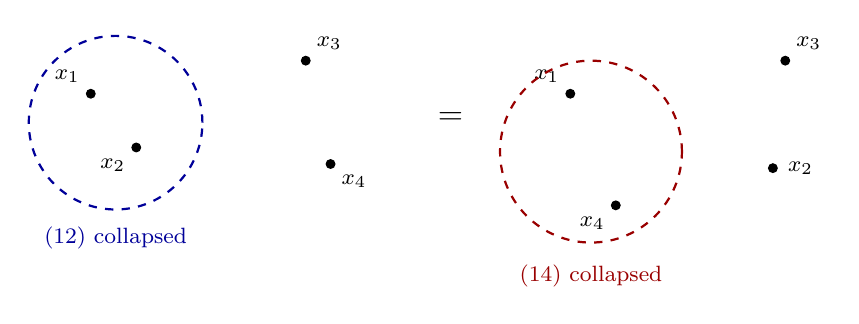
\begin{tikzpicture}[scale=1.05, >=stealth]
  % left: (12)(34) channel
  \begin{scope}
    \filldraw (0.0,0.35) circle (1.5pt) node[above left=0.5pt] {\footnotesize $x_1$};
    \filldraw (0.55,-0.3) circle (1.5pt) node[below left=0.5pt] {\footnotesize $x_2$};
    \filldraw (2.6,0.75) circle (1.5pt) node[above right=0.5pt] {\footnotesize $x_3$};
    \filldraw (2.9,-0.5) circle (1.5pt) node[below right=0.5pt] {\footnotesize $x_4$};
    \draw[dashed, thick, blue!60!black] (0.3,0.0) circle (1.05);
    \node[blue!60!black] at (0.3,-1.4) {\footnotesize $(12)$ collapsed};
  \end{scope}
  % equals sign
  \node at (4.35,0.05) {\large $=$};
  % right: (14)(23) channel
  \begin{scope}[xshift=5.8cm]
    \filldraw (0.0,0.35) circle (1.5pt) node[above left=0.5pt] {\footnotesize $x_1$};
    \filldraw (0.55,-1.0) circle (1.5pt) node[below left=0.5pt] {\footnotesize $x_4$};
    \filldraw (2.6,0.75) circle (1.5pt) node[above right=0.5pt] {\footnotesize $x_3$};
    \filldraw (2.45,-0.55) circle (1.5pt) node[right=2pt] {\footnotesize $x_2$};
    \draw[dashed, thick, red!60!black] (0.25,-0.35) circle (1.1);
    \node[red!60!black] at (0.25,-1.85) {\footnotesize $(14)$ collapsed};
  \end{scope}
\end{tikzpicture}
\caption{Crossing symmetry as two radial quantizations of one correlator:
  expand within the sphere that encloses $(x_1, x_2)$, or within the sphere
  that encloses $(x_1, x_4)$. Where both separating spheres exist, both OPE
  expansions converge --- to the same function. Equation \eqref{eq:crossing}
  is the statement that the bookkeeping cannot depend on the choice.}
\label{fig:crossing}
\end{figure}

% =====================================================================
\subsection{The stress tensor}
\label{sec:stress-tensor}

Stand back and audit what the chapter has assumed about its subject. Analytic
continuation needed a positive Hamiltonian; reconstruction needed reflection
positivity; the OPE needed conformal symmetry on top. Nowhere did we use ---
or even state --- the property chapter I.1 declared the ``one non-negotiable'':
locality. And the omission is not cosmetic. Everything so far would be
satisfied by systems nobody calls a field theory; the sharpest way to see this
is that we will shortly construct, in Example~\ref{ex:gff}, a full set of
conformal, reflection-positive, OPE-convergent correlators describing no local
theory at all. What separates quantum field theory from ``quantum mechanics
with correlators'' must therefore live somewhere specific in the operator
content. Chapter I.1 told us where: in the existence of a local \vocab{stress
tensor} --- the operator that measures energy and momentum \emph{density},
equivalently the response of the theory to local deformations of the geometry
it lives on. This section constructs that operator, extracts the identities
that make it useful, and then exhibits the counterexample that makes it
necessary.

\subsubsection{Definition and Ward identities}

In any presentation with an action on a background metric, the definition is a
functional derivative (we work in Euclidean signature; Lorentzian signs and
the index dictionary are pinned in Appendix~\ref{app:conventions}):
\begin{equation}
T_{\mu\nu}(x) \;\equiv\; \frac{2}{\sqrt{g}}\,
\frac{\delta S_{\rm E}}{\delta g^{\mu\nu}(x)} ,
\label{eq:stress-def}
\end{equation}
the source conjugate to the metric, exactly as a current is the source
conjugate to a background gauge field. The definition looks
presentation-bound --- it mentions an action --- but the structure it
produces is not, and the modern attitude is to take the \emph{output} as the
definition: a local QFT is one possessing a symmetric tensor operator
$T_{\mu\nu}$, of dimension exactly $d$ at a fixed point, satisfying the Ward
identities we now derive.

Insert operators $\op_1(x_1)\cdots\op_n(x_n)$ into the flat-space path
integral and perform an infinitesimal diffeomorphism $x \to x' = x +
\epsilon(x)$, with $\epsilon$ vanishing at infinity, treated as a mere change
of integration variables --- which changes the value of the integral not at
all. Track where the relabeling acts. The measure is invariant (we assume; in
chiral theories this very step can fail, which is one address of the
anomalies of Part II). The action is \emph{not} invariant --- flat space has
no reason to be diffeomorphism-invariant by itself --- but its variation is,
by the definition \eqref{eq:stress-def}, the stress tensor contracted with
the induced metric deformation $\delta g_{\mu\nu} = \partial_\mu
\epsilon_\nu + \partial_\nu \epsilon_\mu$:
\begin{equation}
\delta S_{\rm E}
= \frac12 \int d^dx \; T^{\mu\nu}\, \delta g_{\mu\nu}
= \int d^dx \; T^{\mu\nu}\, \partial_\mu \epsilon_\nu
= -\int d^dx \; \epsilon_\nu \,\partial_\mu T^{\mu\nu} ,
\end{equation}
using the symmetry of $T$ and integrating by parts. And the insertions
transport: a scalar shifts by $\delta_\epsilon \op(x_i) =
\epsilon^\nu(x_i)\, \partial_\nu \op(x_i)$. Since the relabeled integral
equals the original,
\begin{equation}
0 \;=\; -\big\langle\, \delta S_{\rm E}\; \op_1 \cdots \op_n\big\rangle
\;+\; \sum_i \big\langle \op_1 \cdots \delta_\epsilon \op_i \cdots
\op_n\big\rangle ,
\end{equation}
and stripping the arbitrary function $\epsilon^\nu(x)$
gives the local identity
\begin{equation}
\partial_\mu \big\langle T^{\mu\nu}(x)\, \op_1(x_1)\cdots\op_n(x_n)
\big\rangle
\;=\; -\sum_{i=1}^n \delta^d(x - x_i)\;
\frac{\partial}{\partial x_i^{\,\nu}}
\big\langle \op_1(x_1) \cdots \op_n(x_n)\big\rangle .
\label{eq:t-ward}
\end{equation}
(Operators with spin contribute an extra rotation piece, $\propto
\partial_\mu[\delta^d(x - x_i)\, \Sigma^{\mu\nu}]$, which the reader may
restore when needed.) Read \eqref{eq:t-ward} twice; the two readings have
different morals.

\emph{Away from insertions, $T^{\mu\nu}$ is conserved as an operator
equation.} The right-hand side is a sum of contact terms, so at separated
points $\partial_\mu T^{\mu\nu} = 0$ inside any correlator. This is Noether's
theorem in correlator form, with no Lagrangian on stage.

\emph{At insertions, the contact terms make charges act.} Integrate
\eqref{eq:t-ward} against a vector field $\xi^\nu$ over a region $R$ bounded
by a closed surface $\Sigma$. If $\xi$ generates a symmetry of flat space
(translations; or rotations, dilatations, special conformal transformations
when $T$ is symmetric and traceless), the bulk integral collapses to a surface
integral, and one finds
\begin{equation}
\oint_{\Sigma} dS_\mu \; \xi_\nu\, \big\langle T^{\mu\nu}(x)\,
\op_1(x_1)\cdots \big\rangle
\;=\; -\sum_{x_i \in R}
\big\langle \cdots\, \delta_\xi \op_i(x_i)\, \cdots \big\rangle ,
\label{eq:charge-ward}
\end{equation}
where $\delta_\xi \op$ is the operator's transformation. The object
\begin{equation}
Q_\xi[\Sigma] \;=\; \oint_\Sigma dS_\mu\, \xi_\nu \, T^{\mu\nu}
\label{eq:topological-charge}
\end{equation}
is the conserved charge, and \eqref{eq:charge-ward} says something stronger
than conservation: the surface $\Sigma$ can be \emph{deformed at will} without
changing any correlator, as long as no insertion point is crossed --- the
difference of two surface integrals is a bulk integral of
\eqref{eq:t-ward}'s left side, which vanishes away from insertions. The
charges of a local theory are \vocab{topological surface operators}: their
value depends only on which operators they enclose, not on the surface's
shape, size, or location. Crossing an insertion changes the correlator by
exactly the enclosed operator's transformation. These are the first genuinely
topological objects of these notes, and they are the thin end of the wedge
that Part II drives through the whole subject --- there, the logic is
\emph{reversed}, and a symmetry is \emph{defined} as a topological operator,
with \eqref{eq:topological-charge} demoted to the special case in which the
topological operator happens to be built from a local current.

In particular, the conformal generators that powered radial quantization are
charges of exactly this kind --- the loan taken out in
Section~\ref{sec:radial-quantization} can now be repaid. For each conformal
Killing vector of flat space, evaluate \eqref{eq:topological-charge} on a
sphere:
\begin{equation}
\begin{aligned}
P_\mu &= \oint dS_\rho\, T^{\rho}_{\ \mu}\,, &
M_{\mu\nu} &= \oint dS_\rho \big(x_\mu T^{\rho}_{\ \nu} - x_\nu
T^{\rho}_{\ \mu}\big), \\
D &= \oint dS_\rho\; x^\nu\, T^{\rho}_{\ \nu}\,, &
K_\mu &= \oint dS_\rho \big(2 x_\mu x^\nu - \delta_\mu^{\ \nu}
x^2\big)\, T^{\rho}_{\ \nu}\,,
\end{aligned}
\label{eq:conformal-charges}
\end{equation}
the last two conserved surface-independently only because $T$ is traceless
($\xi_\nu T^{\mu\nu}$ has divergence $\tfrac1d (\partial\cdot\xi)\,
T^\mu_{\ \mu}$ for a conformal Killing vector $\xi$). Shrinking the surface
onto an insertion converts \eqref{eq:charge-ward} into the commutator
statement: in radial ordering, $Q_\xi$ just inside minus $Q_\xi$ just
outside an insertion is
\begin{equation}
\big[\, Q_\xi\,,\, \op(x)\,\big] \;=\; \delta_\xi\, \op(x)\,,
\label{eq:charge-commutator}
\end{equation}
which for the choices \eqref{eq:conformal-charges} reproduces exactly the
algebra postulated in Section~\ref{sec:radial-quantization}: $[D, \op(0)] =
\Delta\,\op(0)$, $[P_\mu, \op(x)] = \partial_\mu\op(x)$, and the rest. The
bookkeeping device of radial quantization is thus generated, operator by
operator, by the stress tensor --- which is the precise sense in which
conformal symmetry is a property \emph{of a local theory} rather than of a
coordinate change: no traceless conserved $T$, no charges
\eqref{eq:conformal-charges}, no radial Hamiltonian, no state--operator
correspondence. (The generalized free field below is about to make this
threat concrete: its conformal invariance is real but \emph{global only} ---
inherited from correlator kinematics, with no local generator implementing
it.)

\begin{eexample}[The stress tensor of the free scalar, canonical and improved]
\label{ex:scalar-stress}
For the free massless scalar, the definition \eqref{eq:stress-def} applied to
$S_{\rm E} = \frac12\int \sqrt g\, g^{\mu\nu}\partial_\mu\phi\,\partial_\nu\phi$
gives, in flat space,
\begin{equation}
T_{\mu\nu} \;=\; \partial_\mu \phi\, \partial_\nu \phi
- \frac{1}{2}\,\delta_{\mu\nu}\, (\partial\phi)^2 ,
\label{eq:canonical-T}
\end{equation}
which coincides here with the Noether current of translations: symmetric,
conserved on-shell ($\partial^\mu T_{\mu\nu} = (\partial_\nu \phi)\,
\partial^2\phi$), and --- a problem --- not traceless:
\begin{equation}
T^{\mu}_{\ \mu} = \Big(1 - \frac d2\Big)(\partial\phi)^2 \;\ne\; 0
\quad (d > 2).
\end{equation}
A nonzero trace would, by the argument below, obstruct using
\eqref{eq:topological-charge} to build the dilatation and special conformal
charges --- yet the free massless scalar \emph{is} conformal. The resolution
is that \eqref{eq:stress-def} has a hidden ambiguity: actions that agree in
flat space can disagree about the metric response. Add the non-minimal
coupling $\frac{\xi}{2} \int \sqrt g \, \mathcal{R}\, \phi^2$ ($\mathcal{R}$
the Ricci scalar): it vanishes in flat space, changes no flat-space
correlator, but shifts the stress tensor by an identically conserved
\vocab{improvement term},
\begin{equation}
T_{\mu\nu} \;\longrightarrow\; T_{\mu\nu}
+ \xi \,\big(\delta_{\mu\nu}\,\partial^2 - \partial_\mu \partial_\nu\big)\phi^2 .
\label{eq:improvement}
\end{equation}
The trace of the added piece is $\xi(d-1)\,\partial^2\phi^2 =
2\xi(d-1)\big[(\partial\phi)^2 + \phi\,\partial^2\phi\big]$, so on-shell
\begin{equation}
T^{\mu}_{\ \mu}\Big|_{\rm improved}
= \Big[\Big(1 - \frac d2\Big) + 2\xi(d-1)\Big](\partial\phi)^2
\;=\; 0
\quad\text{for}\quad
\xi_c = \frac{d-2}{4(d-1)} ,
\label{eq:conformal-coupling}
\end{equation}
the \vocab{conformal coupling} ($\xi_c = \frac16$ in $d = 4$; $\xi_c = 0$ in
$d=2$, where \eqref{eq:canonical-T} was traceless on-shell all along ---
another early hint that $d=2$ is special). Three durable lessons. \emph{(i)}
``The'' stress tensor is an equivalence class: improvements
\eqref{eq:improvement} change the operator without changing the charges
$P^\mu$ or the physics, and statements about $T$ should be improvement-aware.
\emph{(ii)} Conformal invariance is the statement that a \emph{traceless}
representative exists; with it, $\xi_\nu T^{\mu\nu}$ is conserved for every
conformal Killing vector $\xi$ (the trace multiplies $\partial\cdot\xi$),
and all the charges of radial quantization flow from
\eqref{eq:topological-charge}. \emph{(iii)} The improved $T$ is the
fixed-point operator: it is the spin-2 primary of dimension $d$ in the free
CFT's spectrum, the operator that the OPE machinery sees (cf.\
Exercise~\ref{exr:free-ope}: the level-$(0,2)$ composite in $\phi \times
\phi$ is exactly \eqref{eq:improvement}-improved).
\end{eexample}

The trace earns its own paragraph, because it is the operator that knows
about scale. Repeating the derivation of \eqref{eq:t-ward} for a \emph{Weyl}
variation $\delta g_{\mu\nu} = 2\omega(x)\, g_{\mu\nu}$ instead of a
diffeomorphism shows that $T^\mu_{\ \mu}(x)$ measures the response to local
rescalings; in a flowing theory the schematic operator equation
\begin{equation}
T^{\mu}_{\ \mu} \;=\; \sum_i \beta^i(g)\; \op_i
\label{eq:trace-beta}
\end{equation}
identifies the trace with the beta functions --- the precise statement, with
its subtleties (operator mixing, ``virial current'' ambiguities), is part of
chapter I.6's honest construction of the RG, and the question of when
$T^\mu_{\ \mu} = 0$ exactly (scale versus conformal invariance) was flagged
already in chapter I.1's theory-space section. Here we need only the fixed-point
moral: at a fixed point a traceless stress tensor exists in all known unitary
local examples, and these notes assume it wherever ``CFT'' is written.

\begin{exercise}[classic]
\label{exr:t-ward-check}
Test the Ward identity \eqref{eq:t-ward} on the free scalar. Using Wick's
theorem with \eqref{eq:canonical-T} improved at $\xi_c$, compute $\langle
T_{\mu\nu}(x)\, \phi(x_1)\,\phi(x_2)\rangle$ in $d=4$ and verify: (a) it is
conserved away from $x_1, x_2$; (b) integrating the $\nu = 0$ component
of \eqref{eq:t-ward} over a ball around $x_1$ reproduces $\partial_{x_1}$
acting on $\langle\phi\phi\rangle$; (c) the same correlator with the
\emph{unimproved} $T$ fails tracelessness by contact terms plus the on-shell
piece, and identify how the dilatation Ward identity then misreports
$\Delta_\phi$.
\hint{Work in momentum space if the contact terms get confusing; or use the
position-space identity $\partial^2 (1/x^2) = -4\pi^2 \delta^4(x)$
repeatedly.}
\end{exercise}

\begin{exercise}[medium]
\label{exr:tt-positivity}
The two-point function of stress tensors in a CFT takes the form $\langle
T_{\mu\nu}(x) T_{\rho\sigma}(0)\rangle = C_T \,\frac{\mathcal{I}_{\mu\nu,
\rho\sigma}(x)}{x^{2d}}$ with $\mathcal{I}$ a fixed tensor structure built
from inversions, and $C_T > 0$ in a unitary theory --- by now you can see why
(it is a norm in radial quantization). Compute $C_T$ for the free conformal
scalar in $d = 4$ by Wick contraction of two improved stress tensors, in any
normalization you state clearly, and check positivity. ($C_T$ will return as
a yardstick: it counts degrees of freedom well enough to order theories, and
appears in the monotonicity discussion of Part IV.)
\hint{Repeated Wick contraction; the real content of the exercise is the
check that the $\xi_c$-dependent pieces assemble into the conserved,
traceless structure $\mathcal{I}$ --- the unimproved tensor's correlator is
not even traceless. Compare your value against the general-$d$ free-scalar
$C_T$ tabulated in Osborn--Petkou, \texttt{hep-th/9307010}, \S3, translating
normalizations carefully (everyone's $C_T$ differs by factors of the sphere
volume).}
\end{exercise}

\subsubsection{A consistent set of correlators with no theory underneath}

Now the promised counterexample, which converts ``the stress tensor is what
makes it a field theory'' from slogan to theorem-adjacent fact. The
construction is almost insultingly simple, and that is its point.

\begin{eexample}[The generalized free field]
\label{ex:gff}
Pick a number $\Delta \ge \frac{d-2}{2}$ and \emph{declare} a scalar operator
$\op$ with two-point function
\begin{equation}
\langle \op(x)\,\op(0)\rangle = \frac{1}{x^{2\Delta}},
\end{equation}
and all higher correlators given by Wick's theorem --- sums over pairings of
products of two-point functions, exactly as for a Gaussian field:
\begin{equation}
\langle \op(x_1)\op(x_2)\op(x_3)\op(x_4)\rangle
= \frac{1}{x_{12}^{2\Delta}x_{34}^{2\Delta}}
+ \frac{1}{x_{13}^{2\Delta}x_{24}^{2\Delta}}
+ \frac{1}{x_{14}^{2\Delta}x_{23}^{2\Delta}},
\qquad \text{etc.}
\label{eq:gff-4pt}
\end{equation}
This is the \vocab{generalized free field} (GFF; ``mean field theory'' in
bootstrap dialect). Run the chapter's checklist against it, and watch every
single axiom pass:

\emph{Euclidean covariance, permutation symmetry, clustering:} immediate from
the form of \eqref{eq:gff-4pt}. In fact the correlators are covariant under
the full \emph{conformal} group, since the two-point function is and Wick
products inherit it.

\emph{Reflection positivity:} a Gaussian theory is reflection positive iff its
covariance is, and Section~\ref{sec:kallen-lehmann} already did the
computation: the K\"all\'en--Lehmann density of $1/x^{2\Delta}$ is the
positive function \eqref{eq:cft-spectral} precisely when $\Delta \ge
\frac{d-2}{2}$. So the OS reconstruction of
Section~\ref{sec:os-reconstruction} runs without complaint and produces an
honest Hilbert space --- a Fock space generated by $\op$, with a positive
Hamiltonian, a unitary conformal group, the lot.

\emph{OPE and its convergence:} by Wick algebra,
\begin{equation}
\op(x)\,\op(0) = \frac{1}{x^{2\Delta}}\cdot\mathbf 1
+ :\!\op^2\!:(0) + \cdots,
\end{equation}
and the full single-$\op$-pair spectrum consists of the \vocab{double-twist}
composites
\begin{equation}
[\op\op]_{n,\ell} \;\sim\;\,
:\!\op\;\partial^{2n}\partial_{\mu_1}\!\cdots\partial_{\mu_\ell}\,\op\!: \,,
\qquad
\Delta_{n, \ell} = 2\Delta + 2n + \ell ,
\qquad \ell \text{ even},
\label{eq:double-twist}
\end{equation}
an integer-spaced tower starting at $2\Delta$. The four-point function
\eqref{eq:gff-4pt} decomposes into these multiplets with computable, positive
squared OPE coefficients (Exercise~\ref{exr:gff-ope}), the expansion
converging exactly as Theorem~\ref{thm:ope-convergence} dictates. Crossing
symmetry --- the bootstrap's one dynamical equation --- holds by inspection:
\eqref{eq:gff-4pt} is manifestly symmetric under permuting the points.

\emph{And yet there is no stress tensor.} The complete list of primaries is
$\mathbf 1$, $\op$, and the towers $[\op\cdots\op]_{n,\ell}$ built on
\eqref{eq:double-twist} and its multi-$\op$ generalizations. A stress tensor
must be a spin-2 primary of dimension exactly $d$. The spin-2 candidates
available have dimensions $2\Delta + 2n + 2$ and up: for generic $\Delta$,
\emph{no operator of dimension $d$ exists at all}, and the lone exception
\begin{equation}
2\Delta + 2 = d
\quad\Longleftrightarrow\quad
\Delta = \frac{d-2}{2}
\end{equation}
is the free scalar, where $[\op\op]_{0,2}$ is precisely the improved tensor
of Example~\ref{ex:scalar-stress}. The same counting kills conserved
currents: a spin-1 double-twist would need $2\Delta + 1 = d - 1$, free field
again. (For a single real $\op$ the odd-spin double-twists are absent as
primaries --- $[\op\op]_{0,1} \sim\, :\!\op\,\partial\op\!: =
\tfrac12\partial\,{:}\op^2{:}$ is a descendant --- so strictly this is the
\emph{complex} GFF's verdict, where the $\op^\dagger\op$ tower supplies the
spin-1 candidate; either way no current of dimension $d-1$ survives off the
free point.) The moment $\Delta$ moves off the free value, the theory keeps every
correlator-level virtue --- unitarity, conformal symmetry, convergent
operator algebra, crossing --- and loses energy density, momentum density,
and local charge density. There is no Hamiltonian \emph{density}; only the
global charges survive (they act fine on Fock space). By the standard of
Idea~\ref{idea:locality}, this is not a quantum field theory. It is the
quantum mechanics of a conformally organized continuum of oscillators.
\end{eexample}

Two reflections on the example, one structural, one physical. Structurally,
notice \emph{where} the failure lives: not in any correlator you could
falsify locally, but in the \emph{absence} of an operator --- a hole in the
spectrum at spin 2, dimension $d$. No finite list of correlator measurements
detects it; you must know the whole operator content to know the theory is
nonlocal. This sharpens chapter I.1's Idea~\ref{idea:observables}: ``the
theory is its observables'' means the \emph{complete} assignment, including
which operators exist, not any finite sample of correlators --- and it
forewarns of chapter I.3, where theories agreeing on \emph{all} local
correlators will differ in their extended operators. It also matters
practically: the numerical bootstrap must \emph{input} the existence of a
stress tensor (or not) as a hypothesis, exactly because crossing alone is
satisfied by GFF-like solutions --- the bootstrap's exclusion plots are
maps of where local theories can live inside the larger continent of
crossing-symmetric data.

Physically, the GFF is anything but pathological --- it is ubiquitous,
appearing whenever a local theory is viewed through a nonlocal window.
It is the boundary description of a \emph{free field in $(d+1)$-dimensional
anti-de Sitter space} (the extra dimension is where the missing locality
went --- and where the stress tensor lives: AdS gravity off), the kinematic
skeleton on which holography is built in Part XI. It is the strict large-$N$
limit of correlators of single-trace operators (factorization = Wick's
theorem, cf.\ Part XI.1). And it is the actual critical theory of the
long-range Ising model in part of its phase diagram --- the system chapter
I.1 used to illustrate locality's failure modes, now revealed as a GFF in
the flesh.\footnote{For GFF as AdS boundary data see Penedones's TASI
lectures \arxiv{1608.04948}; for the long-range Ising application, Rychkov
\arxiv{1601.05000}, \S1.3.2. The double-twist spectrum
\eqref{eq:double-twist} is the starting point of the large-spin analytic
bootstrap (Part III.3), which quantifies the statement that \emph{every} CFT
approaches GFF behavior at large spin.}

\begin{nnote}
``Generalized \emph{free} field'' refers to Wick factorization, not to a
Lagrangian: away from the free value of $\Delta$ no local action in $d$
dimensions produces these correlators --- the would-be kinetic operator is a
fractional power of the Laplacian, meaningful only as an integral
kernel. The GFF is the cleanest standing illustration that the
space of consistent ``correlator systems'' is strictly larger than the space
of local QFTs, with the stress tensor as the membership card.
\end{nnote}

\begin{exercise}[classic]
\label{exr:gff-ope}
Decompose the GFF four-point function. With $u, v$ the standard cross-ratios,
show from \eqref{eq:gff-4pt} that the $(12)(34)$-channel expansion contains
the identity plus double-twist towers, and compute the squared OPE coefficient
of the leading scalar $[\op\op]_{0,0} = \tfrac{1}{\sqrt 2}:\!\op^2\!:$
(answer: $\lambda^2 = 2$ in unit-normalized conventions). Verify positivity
of the first few coefficients, and check that the spin-2, $n=0$ coefficient
stays finite and nonzero as $\Delta \to \frac{d-2}{2}$ --- the stress tensor
re-entering the spectrum continuously.
\hint{Expand $u^{\Delta}(1 + v^{-\Delta})$-type terms in the small-$u$,
small-$1-v$ limit and match powers against the leading conformal block
behavior $u^{\Delta_{n,\ell}/2}$; the systematic closed form for all $n,
\ell$ is in the literature (Fitzpatrick--Kaplan--Poland--Simmons-Duffin), but
the leading entries are a half-page of algebra.}
\end{exercise}

\begin{exercise}[thinker]
\label{exr:gff-lattice}
Could any \emph{local} lattice model --- finite-range couplings, finite-
dimensional on-site spaces --- flow to the GFF with $\Delta \ne
\frac{d-2}{2}$ at criticality? Marshal the evidence from this section
(existence of $T$ on the lattice side? what happens to it in the limit?) and
from chapter I.1's locality discussion. Then reconcile with the fact that the
\emph{long-range} Ising model does reach it. What exactly about
$J_{ij} \sim |i-j|^{-d-\sigma}$ evades your argument?
\hint{A local lattice model has a (lattice) energy density whose continuum
limit, if the limit is a CFT, supplies a stress tensor candidate; the
long-range model's energy density is not local. This is heuristic --- making
it a theorem is open territory; see the discussion of stress-tensor
existence in Rychkov \arxiv{1601.05000}, \S1.3.2.}
\end{exercise}

% =====================================================================
\subsection{Conserved currents and their products}
\label{sec:currents}

The stress tensor is the local operator that every local theory must have. A
theory with global symmetry has, in the same spirit, one more universal
piece of operator content per continuous symmetry: a conserved \vocab{current}
$J^\mu$, the source conjugate to a background gauge field as $T_{\mu\nu}$ is
conjugate to the metric. The change-of-variables argument that produced
\eqref{eq:t-ward} transcribes line for line --- with an $x$-dependent
symmetry rotation in place of the diffeomorphism. Let the symmetry act on
charged operators as $\op_k \to e^{iq_k\alpha}\,\op_k$ with constant
$\alpha$; promote $\alpha \to \alpha(x)$ and relabel the path integral. The
action is not invariant under the local version, and its leading variation
\emph{defines} the current,
\begin{equation}
\delta S_{\rm E} \;=\; -i\int d^dx \;J^\mu(x)\, \partial_\mu \alpha(x)\,,
\end{equation}
while each insertion rotates by its charge, $\delta\op_k = i q_k\,
\alpha(x_k)\,\op_k$. Equating the two and stripping $\alpha(x)$ yields the
current's Ward identity,
\begin{equation}
\partial_\mu \big\langle J^{\mu}(x)\,\op_1(x_1)\cdots\op_n(x_n)\big\rangle
\;=\; \sum_{k} q_k\; \delta^d(x - x_k)\,
\big\langle \op_1(x_1)\cdots\op_n(x_n)\big\rangle ,
\label{eq:j-ward}
\end{equation}
with the same two morals as before: conservation as an
operator equation at separated points, and charges
\begin{equation}
Q[\Sigma] = \oint_\Sigma dS_\mu \, J^\mu
\label{eq:current-charge}
\end{equation}
that are \emph{topological surface operators} --- deformable freely until they
cross a charged insertion, at which moment the correlator jumps by $q_k$.
Conservation also rigidly fixes kinematics at a fixed point: a conserved
vector primary must have dimension exactly $\Delta_J = d - 1$ (and conversely,
a vector primary at the unitarity-bound dimension $d-1$ is automatically
conserved --- Exercise~\ref{exr:current-dimension}), with two-point function
\begin{equation}
\langle J_\mu(x)\, J_\nu(0)\rangle
= C_J\, \frac{I_{\mu\nu}(x)}{x^{2(d-1)}},
\qquad
I_{\mu\nu}(x) = \delta_{\mu\nu} - \frac{2 x_\mu x_\nu}{x^2},
\qquad C_J > 0.
\label{eq:jj-2pt}
\end{equation}

So far this is the stress-tensor story with one index fewer, and we could
leave it there. The reason for a separate section --- and for this chapter to
end on it --- is that the \emph{products} of currents carry structure that no
single current sees, and that structure turns out to be among the most rigid,
most quantized, most RG-stable data in all of quantum field theory. The
slogan to hold: \emph{a current is kinematics; current algebra is dynamics}.
Three exhibits, in ascending order of consequence.

\emph{The $JJ$ OPE knows about locality.} In a local theory the product
$J_\mu(x) J_\nu(0)$ expands, by Theorem~\ref{thm:ope-convergence}, in the
theory's operator content --- and the stress tensor, when it exists, appears
in this OPE with a coefficient fixed by the Ward identity
\eqref{eq:t-ward} in terms of $C_J$: energy density couples universally to
everything charged. (In the GFF-with-current variants, the term is simply
absent --- the hole in the spectrum again.)

\emph{The $JJJ$ correlator knows about anomalies.} In even dimensions, the
three-point function of currents contains, alongside its conformally trivial
parts, a parity-odd contact structure whose coefficient is the \vocab{'t
Hooft anomaly} of the symmetry --- the famous triangle diagram of $d=4$
textbooks, reborn as a statement about an exactly computable, position-space
correlator of the abstract theory. We say no more here, because Part II.3
builds anomaly technology properly; but the address is worth recording now:
\emph{anomalies live in current correlators}, which is why they survive every
RG flow that preserves the symmetry --- correlators of conserved currents at
separated points cannot jump along a continuous flow.

\emph{And already the $JJ$ commutator hides a quantized term that no
classical reasoning produces.} This is the Schwinger term, the chapter's
closing calculation, and a fitting one: it uses the analytic structure of
Section~\ref{sec:analytic-structure}, the positivity of
Section~\ref{sec:reflection-positivity}, and the operator-content reasoning
of this section, all at once --- and it is the first appearance in these
notes of a phenomenon (a central, quantized obstruction in a symmetry
algebra) that Part II will industrialize.

\begin{eexample}[The Schwinger term]
\label{ex:schwinger-term}
The claim, first the shock value: in any unitary theory with a nontrivial
$U(1)$ symmetry, the equal-time commutator of charge density with current
density \emph{cannot vanish},
\begin{equation}
\big[\, J^0(\mathbf{x})\,,\, J^i(\mathbf{y})\,\big]_{\rm equal\ time} \;\ne\; 0,
\end{equation}
even though the naive canonical computation, in essentially every
presentation, gives zero. Worse for the naive computation: in $d = 2$ the
nonvanishing piece is a c-number with a \emph{quantized} coefficient.

\emph{The no-go (Schwinger's positivity argument, any $d$).} Suppose the
commutator vanished. Smear the charge density against a real profile $f$,
$J^0(f) = \int d^{d-1}x\, f(\mathbf{x})\, J^0(0,\mathbf{x})$, and consider
\begin{equation}
\mathcal{C}_f \;\equiv\;
\bra{0}\big[\, J^0(f)\,,\, [\, H\,,\, J^0(f)\,]\big]\ket{0}
\;=\; 2\sum_n E_n\, \big|\bra{n} J^0(f)\ket{0}\big|^2 \;\ge\; 0,
\label{eq:schwinger-positivity}
\end{equation}
by inserting a complete set of states --- positivity of the energy and of
norms, doing the work one more time. But current conservation trades the
inner commutator for the spatial current, $[H, J^0] = -i\,\partial_t J^0 =
+i\,\partial_i J^i$, so $\mathcal{C}_f$ is built entirely from the equal-time
$[J^0, J^i]$ --- which we assumed to vanish. Then \emph{every} state created
from the vacuum by the charge density has zero amplitude, $J^0(f)\ket{0} = 0$
for all $f$; and a local operator that annihilates the vacuum annihilates
everything (vacuum cyclicity --- Exercise~\ref{exr:reeh-schlieder}), so
$J^\mu \equiv 0$. A nontrivial symmetry therefore \emph{requires} a nonzero
equal-time $[J^0, J^i]$: a ``Schwinger term,'' invisible to canonical
manipulations, mandated by unitarity.\footnote{J.~Schwinger, Phys.\ Rev.\
Lett.\ \textbf{3} (1959) 296; the term had been noticed by Goto and Imamura
in 1955. The canonical computation misses it because the product of two
currents at coincident points is singular --- exactly the singularity the
OPE organizes --- and manipulating it as if fields were smooth drops the
central piece.}

\emph{The exact computation ($d = 2$).} Now compute the term, in the cleanest
habitat: a 2d CFT with a $U(1)$ current --- the compact boson, or the
massless Dirac fermion at level $k = 1$. Conservation plus tracelessness
split the current into chiral halves; take the right-mover $j(x^-)$, $x^\pm =
x \pm t$, with Wightman two-point function normalized by the level,
\begin{equation}
\bra{0} j(x)\, j(0) \ket{0}
\;=\; \frac{k}{4\pi^2}\,\frac{1}{(x^- - i\epsilon)^2}\,,
\label{eq:jj-2d}
\end{equation}
the $i\epsilon$ encoding, as always, the boundary value from the
positive-energy domain. The equal-time commutator is the jump between the two
boundary values --- the tool of Example~\ref{ex:free-scalar-2pt}, reused
verbatim. With the Sokhotski formula $\frac{1}{(x \mp i\epsilon)^2} = -
\frac{d}{dx}\big(\mathrm{P}\frac1x \pm i\pi\,\delta(x)\big)$,
\begin{equation}
\bra{0}\big[\,j(x)\,,\,j(0)\,\big]\ket{0}\Big|_{t=0}
= \frac{k}{4\pi^2}\left[\frac{1}{(x-i\epsilon)^2} -
\frac{1}{(x+i\epsilon)^2}\right]
= -\,\frac{i k}{2\pi}\;\delta'(x).
\label{eq:schwinger-2d}
\end{equation}
For an abelian current algebra the commutator is a pure c-number, so
\eqref{eq:schwinger-2d} is the full operator statement: $[\,j(x), j(y)\,] =
-\frac{ik}{2\pi}\,\delta'(x-y)$. Assembling $J^0 = j_+ + j_-$, $J^1 = j_+ -
j_-$ from the two chiralities (the left-mover's central term carries the
opposite sign) gives the advertised $[J^0(x), J^1(y)] = -\frac{ik}{\pi}\,
\delta'(x - y)$, while the charge-density commutator $[J^0, J^0]$ cancels
between chiralities, as consistency demands. Smear the chiral current into
charges, $Q_f \equiv \int dx\, f(x)\, j(x)$, and the result reads as algebra:
\begin{equation}
\big[\, Q_f \,,\, Q_g \,\big] \;=\; \frac{ik}{2\pi} \int dx\; f'(x)\, g(x)\,,
\label{eq:central-extension}
\end{equation}
antisymmetric under $f \leftrightarrow g$ (integrate by parts) and immune to
any redefinition of the charges by c-numbers: the algebra of chiral $U(1)$
transformations is realized on the Hilbert space only up to a \vocab{central
extension}, with central charge $k$. The constant charge $f = 1$ commutes
with everything --- the global symmetry is intact --- but the
\emph{local} structure of the symmetry is deformed, and irreparably so. The
particle on a circle at $\theta = \pi$ (chapter I.1) showed a symmetry
realized projectively on a two-state system; here is the field-theory
version, a projective phase per mode, quantified by one integer.

\emph{Why $d=2$ is the sweet spot: the sum rule.} The spectral representation
of Section~\ref{sec:kallen-lehmann}, run for the conserved current, makes the
dimension-dependence of all this quantitative. Conservation forces the
current's two-point function into a transverse form with a single spectral
density $\rho_J(s) \ge 0$, and retracing the boundary-value computation that
produced \eqref{eq:schwinger-2d} --- now mass level by mass level --- one
finds that the Schwinger term is the \emph{total spectral weight}
(Schwinger's original form of the result):
\begin{equation}
\big[\,J^0(\mathbf{x})\,,\,J^i(\mathbf{y})\,\big]_{\rm equal\ time}
\;=\; -\,i\,c\;\partial_i\,\delta^{d-1}(\mathbf{x} - \mathbf{y})\,,
\qquad
c \;\propto\; \int_0^\infty ds\;\rho_J(s) \;>\;0\,.
\label{eq:schwinger-sum-rule}
\end{equation}
Positivity of $\rho_J$ re-derives the no-go at a glance --- a sum of positive
terms cannot vanish unless every term does, i.e.\ unless the current creates
nothing from the vacuum. And the integral diagnoses the dimensions:
dimensional analysis gives the coefficient $c$ mass dimension $d-2$, and
indeed in a CFT $\rho_J(s) \sim C_J\, s^{(d-4)/2}$, whose integral diverges
at large $s$ for every $d > 2$ --- there the Schwinger term is
cutoff-dominated, the famously ``regularization-dependent'' object of the
1960s literature, physical in origin but not a number you can quote. In
$d = 2$, and only there, the density of a conserved current is an integrable
$\rho_J(s) = k\,\delta(s)$ and the sum rule converges: the Schwinger term is
a \emph{pure number}, $k$ --- universal, quantized (for a compact symmetry
--- Part III.4 derives the integrality), and the first member of the new
canon of exact coefficients these notes collect. The reader has, in fact, just computed three things at once: the
central extension of the $U(1)$ current algebra (the Kac--Moody level, the
backbone of 2d CFT in Part III.4); the 't Hooft anomaly of the $U(1)$
symmetry in $d=2$ (couple $j$ to a background field and
\eqref{eq:schwinger-2d} obstructs gauge invariance --- the two-dimensional
sibling of the ABJ triangle, here one line of algebra); and the engine of
the Schwinger model, where this commutator is what generates the photon mass
$e/\sqrt\pi$ (Part V.4 solves it). One calculation, three previews ---
current \emph{products} are where the exact structure of QFT concentrates.
\end{eexample}

\begin{ppreview}[From currents to Part II]
This section's two findings --- charges are topological surface operators;
current products carry quantized, RG-inert coefficients --- are the embryo of
the symmetry revolution that occupies Part II. There, the topological
surface operator becomes the \emph{definition} of symmetry (no current
needed: discrete symmetries get operators too, with \eqref{eq:current-charge}
the special ``Noether case''), and the quantized coefficients in current
correlators become 't Hooft anomalies, classified and matched along RG flows.
When Part II.1 opens by ``running Noether's theorem backwards,'' it is this
section run backwards.
\end{ppreview}

\begin{exercise}[medium]
\label{exr:current-dimension}
(a) Show that in a CFT, conservation $\partial^\mu J_\mu = 0$ forces $\Delta_J
= d-1$: apply the special-conformal commutator $[K_\nu, \cdot]$ to the
conservation equation for a vector primary and find that consistency requires
either $\Delta = d - 1$ or $\partial^\mu J_\mu \neq 0$. (b) Conversely, show
the two-point function \eqref{eq:jj-2pt} with general power $2\Delta$ in the
denominator is conserved only at $\Delta = d-1$. (c) Conclude the modern
restatement of ``the current does not renormalize'': conservation is not a
property protected by perturbative miracles but a representation-theoretic
fact about the fixed point --- short multiplets stay short. (The same
argument with one more index pins $\Delta_T = d$.)
\hint{For (b), brute force: $\partial^\mu [I_{\mu\nu}(x)\, x^{-2\Delta}] =
2(\Delta - d + 1)\, x_\nu\, x^{-2\Delta - 2}\cdot(\dots)$.}
\end{exercise}

\begin{exercise}[medium]
\label{exr:sum-rule}
(The sum rule, checked where it converges.) (a) In $d = 2$, show that
conservation and Lorentz invariance force $\langle J_\mu(p) J_\nu(-p)\rangle
= \big(\delta_{\mu\nu} - \frac{p_\mu p_\nu}{p^2}\big)\,\Pi(p^2)$ with $\Pi$
\emph{constant} for a CFT current, and that the corresponding spectral
density is $\rho_J(s) \propto k\,\delta(s)$: the conserved current of a 2d
CFT creates exactly one massless mode. (b) Insert this density into the
sum rule \eqref{eq:schwinger-sum-rule} and recover the coefficient of
\eqref{eq:schwinger-2d}, fixing the proportionality constants in your
conventions. (c) For the free Dirac fermion in $d = 4$, estimate
$\rho_J(s)$ at large $s$ from the free-field two-point function and verify
that the sum rule diverges quadratically --- reproducing, from pure
spectral positivity, the old result that the $d=4$ Schwinger term is
cutoff-dominated.
\hint{For (a): a $p$-independent transverse structure has its only
discontinuity at $p^2 = 0$. The massless pole is physical: it is the dual
photon/compact-boson mode, and its inevitability in 2d is one route to
bosonization (Part V.4).}
\end{exercise}

\begin{exercise}[thinker]
\label{exr:reeh-schlieder}
(Vacuum cyclicity, the step the no-go borrowed.) The Schwinger argument used:
a local operator satisfying $A(f)\ket 0 = 0$ for all smearings $f$ supported
in some open region vanishes identically. Make this plausible with the
chapter's tools: if $A(f)\ket{0} = 0$, then $\bra 0 \op_1(x_1)\cdots
\op_n(x_n) A(y)\ket 0 = 0$ for $y$ in the region; use the analyticity of
Wightman functions in the times (Section~\ref{sec:analytic-structure}) to
argue the correlator vanishes for \emph{all} $y$, hence $A$ has vanishing
correlators with everything, hence $A = 0$ (as an operator on the vacuum
sector). This is the germ of the Reeh--Schlieder theorem --- ``the vacuum is
cyclic and separating for local algebras'' --- whose precise form, and whose
startling implications for entanglement in QFT, open Part X.
\hint{A holomorphic function vanishing on an open subset of the boundary of
its domain (here: an open set of real points) vanishes identically ---
Figure~\ref{fig:complex-time}'s logic, run in reverse.}
\end{exercise}

% =====================================================================
\subsection{Where this leaves us}
\label{sec:ch2-closing}

The title's claim is earned. Local operators entered this chapter as the
inventory's oldest line item; they leave as primary data: the local operator
content of a quantum field theory determines its Hilbert space, its
Hamiltonian, its symmetries down to their finest quantized coefficients, and
its response to the geometry it lives on --- and in a conformal theory, where
there is no S-matrix, correlators of local operators are not merely
observables but the only observables there are. The three debts of the
opening are paid; it is worth restating by what mechanism, because each
clause of the verdict was a section.

A correlator is one analytic object viewed from several real slices: the
statistical averages of a Euclidean presentation and the ordered amplitudes
of quantum mechanics are connected by continuation through a domain that
exists because energy is positive --- and the domain of \emph{backgrounds} on
which any of this makes sense is itself charted (Kontsevich--Segal), with
Lorentzian spacetimes on its boundary. Correlators with reflection positivity
\emph{are} a theory: Hilbert space, Hamiltonian, and operators are
constructed from them, by a procedure (Osterwalder--Schrader) whose
sphere-adapted version (radial quantization) converts, in a CFT, the
completeness of the state space into the convergent operator product
expansion --- collapsing the infinite tower of correlators onto the CFT data
$\{\Delta_i, \lambda_{ijk}\}$ with exponentially controlled error. And the
local operator content is not an amorphous list: it is required to contain
the stress tensor and the symmetry currents --- the operators through which
geometry and symmetry act, whose existence is locality's signature
(the generalized free field showing what their absence costs), and whose
products hide the quantized coefficients (Schwinger terms, anomalies) that
survive everything.

What the local data does \emph{not} do is exhaust the observables --- the
title says \emph{Observables I} advisedly. The chapter leaves three loose
threads, deliberately. The charges
\eqref{eq:topological-charge} and \eqref{eq:current-charge} are topological
operators of dimension $d-1$ --- are there others, not generated by any
current? (Part II's affirmative answer reorganizes the subject.) Two theories
can share all local correlators on $\reals^d$ and differ --- chapter I.1's
Exercise~\ref{exr:two-theories-same-correlators} previewed it, and the
missing data lives in operators supported on lines, surfaces, and boundaries:
the extended operators of chapter I.3, next. And the Hilbert spaces this
chapter built on planes and spheres were extracted from correlators ---
chapter I.4 turns the tables and takes the assignment
\emph{geometry $\mapsto$ states} as primary, with cutting and gluing as the
organizing axiom and the state--operator correspondence as its first theorem.
The inventory of chapter I.1 is being filled in, one column at a time.

% =====================================================================
\subsection*{Chapter exercises}

\begin{exercise}[classic]
\label{exr:kms}
(Thermal correlators and the KMS condition.) Compute the two-point function
of the free massless scalar in $d=4$ at temperature $T = 1/\beta$ --- i.e.\
on the Euclidean cylinder $S^1_\beta \times \reals^3$ --- by summing images
over the thermal circle. Show: (a) the Euclidean correlator is periodic in
$\tau$ with period $\beta$; (b) upon continuation to real time, periodicity
becomes the KMS relation $\langle \op(t)\op(0)\rangle_\beta = \langle
\op(0)\op(t - i\beta)\rangle_\beta$ --- the thermal replacement for the
spectral condition, with the strip $-\beta < \mathrm{Im}\, t < 0$ replacing
the half-plane of Figure~\ref{fig:complex-time}. (Thermal states and KMS
return in chapter I.4; the algebraic reformulation is a pillar of Part X.)
\hint{$\sum_{n\in\ints} \frac{1}{r^2 + (\tau + n\beta)^2}$ is summable in
closed form: $\frac{\pi}{r\beta}\,
\frac{\sinh(2\pi r/\beta)}{\cosh(2\pi r/\beta) - \cos(2\pi \tau/\beta)}$.
Check the $\beta\to\infty$ limit.}
\end{exercise}

\begin{exercise}[medium]
\label{exr:cylinder-spectrum}
(The OPE convergence rate is a spectral gap.) For the 2d Ising CFT, the three
lowest primaries are $\mathbf 1$, $\sigma$ ($\Delta = 1/8$), and $\epsilon$
($\Delta = 1$). Using Theorem~\ref{thm:ope-convergence}, estimate how many
multiplets of the $\sigma\times\sigma$ OPE are needed to compute the
four-point function $\langle\sigma\sigma\sigma\sigma\rangle$ to $1\%$
accuracy at the fully symmetric configuration (cross-ratio $z = \bar z =
1/2$, where $e^{-\beta} = 3 - 2\sqrt 2 \approx 0.17$ in the optimal
``$\rho$-coordinate'' frame). Compare with the exactly known answer
(this correlator is solvable; Part III.4): how sharp is the bound?
\hint{Tail $\sim \Delta_*^{4\Delta_\sigma} e^{-\Delta_* \beta}/
\Gamma(4\Delta_\sigma + 1)$ with $\beta = -\log(3 - 2\sqrt2) \approx 1.76$;
the answer is ``embarrassingly few.'' The $\rho$-coordinate refinement is
\arxiv{1208.6449}, \S5.}
\end{exercise}

\begin{exercise}[medium]
\label{exr:gff-reconstruction}
Run the OS reconstruction explicitly for the generalized free field: show
that the Hilbert space built by Steps 1--2 of
Section~\ref{sec:os-reconstruction} from the Wick correlators is the Fock
space over the single-particle space with inner product given by the
two-point function, and identify the reconstructed Hamiltonian's spectrum.
Where, concretely, would you look in this construction for a sign that the
theory is nonlocal --- and fail to find one?
\hint{Gaussian correlators reconstruct Gaussian Hilbert spaces; the
construction never asks whether a stress tensor exists. Locality of the
\emph{dynamics} (Hamiltonian = integral of a density) is simply never
queried by the planar reconstruction.}
\end{exercise}

\begin{exercise}[classic]
\label{exr:current-block}
(The current's place in the operator algebra.) In the 2d free Dirac CFT,
verify by Wick contraction that the $j \times j$ OPE is
\begin{equation*}
j(z)\, j(0) \;=\; \frac{k}{4\pi^2 z^2}
\;+\; \big(\text{stress-tensor term}\big) + \cdots,
\qquad k = 1,
\end{equation*}
(any self-consistent normalization accepted --- state yours), confirming on
this example the general claim that $T$ appears in the $JJ$ OPE of a local
theory with strength tied to $C_J$. Then check the Schwinger-term
computation \eqref{eq:schwinger-2d} directly from fermionic Wick contractions
at equal time, watching the central term arise from the \emph{normal-ordering
subtraction} --- the canonical computation's discarded piece, recovered.
\hint{$j \sim\; :\!\psi^\dagger \psi\!:$ with $\langle \psi(z)
\psi^\dagger(0)\rangle = \frac{1}{2\pi z}$; the double contraction gives the
$z^{-2}$ central term, the single contractions the operator terms.}
\end{exercise}

\begin{exercise}[thinker]
\label{exr:data-vs-theory}
(How much of the theory is the local data, really?) Suppose two unitary
CFTs have identical local CFT data: the same primaries, dimensions, and OPE
coefficients, hence --- by this chapter --- identical correlators of local
operators on $\reals^d$. Catalogue what could still distinguish them, using
only concepts already introduced in Part I (partition functions on other
geometries, item~1 of Definition~\ref{def:inventory}; extended operators,
item~4; the global form of symmetry groups, chapter I.1's
Exercise~\ref{exr:two-theories-same-correlators}). For one concrete handle:
the torus partition function is a sum over the \emph{full} Hilbert space ---
must that Hilbert space be exhausted by the states this chapter constructed
from local operators? (No: chapter I.3's defect Hilbert spaces and chapter
I.4's geometric axiomatics make the gap precise; in 2d, modular invariance
ties the torus to the sphere data and the question becomes sharp ---
Part III.4.)
\end{exercise}

% =====================================================================
\subsection*{Reading}

\begin{description}
\item[Rychkov, \emph{EPFL Lectures on CFT in $D \ge 3$}, \arxiv{1601.05000},
chs.\ 1--3.] The backbone of this chapter's second half: fixed-point
phenomenology and the continuous spectrum (ch.\ 1), radial quantization,
reflection positivity, and the OPE (ch.\ 3). Short, opinionated, and the
natural bridge to Part III.
\item[Simmons-Duffin, \arxiv{1602.07982}, \S\S6--7.] \emph{TASI Lectures on
the Conformal Bootstrap} --- our conventions source. The state--operator
correspondence done carefully via path-integral surgery, Euclidean
conjugation demystified, unitarity bounds; appendix B is a compact summary of
the Euclidean/Lorentzian dictionary.
\item[Pappadopulo et al., \arxiv{1208.6449}.] (Pappadopulo--Rychkov--Espin--%
Rattazzi.) The convergence paper behind Section~\ref{sec:ope-convergence}:
the Cauchy--Schwarz argument, the Hardy--Littlewood spectral estimates, the
exponential rate, and the $\rho$-coordinate optimization. Twenty readable
pages; read it whole.
\item[Kontsevich--Segal, \arxiv{2105.10161}, \S2.] The domain of allowable
complex metrics: Definition 2.1, Theorem 2.2 (our Theorem~\ref{thm:ks}), and
the Lorentzian-on-the-boundary picture. \S\S3 and 5 belong to chapter I.4.
\item[Dedushenko, \arxiv{2203.08053}, \S2.1.] The Wightman and
Osterwalder--Schrader axiom systems with full references --- the rigorous
spine under Sections~\ref{sec:analytic-structure}
and~\ref{sec:reflection-positivity}, including the growth-condition history
this chapter only flagged.
\item[Wilson (1969); Schwinger (1959).] The primary sources for the
chapter's two named structures: the operator algebra as a definition of
dynamics (Phys.\ Rev.\ \textbf{179}, 1499), and the commutator term that
unitarity refuses to waive (Phys.\ Rev.\ Lett.\ \textbf{3}, 296). Both are
short, and both are still worth reading in the original.
\item[Books (for the shelf):] Streater--Wightman, \emph{PCT, Spin and
Statistics, and All That} --- the Wightman axioms and reconstruction, the
spin-statistics and CPT theorems, in 200 pages of permanent value;
Glimm--Jaffe, \emph{Quantum Physics} (already on chapter I.1's shelf) ---
reflection positivity and reconstruction done constructively; Haag,
\emph{Local Quantum Physics} --- the algebraic tradition's summa, background
for Part X.
\end{description}
